% !TEX TS-program = xelatex
% !BIB program = biber
% !TEX encoding = UTF-8 Unicode

% 使用手冊請見 TW_Thesis_Template wiki:
% https://github.com/sppmg/TW_Thesis_Template/wiki

% User guide in wiki of TW_Thesis_Template :
% https://github.com/sppmg/TW_Thesis_Template/wiki

\documentclass[oneside]{NCU_thesis} % \documentclass[option1, option2, ...]
% Helpful options: 
% draft = Don't load figure ,reduce compile time.
% showframe = show document margins.
% colorgrid = show colored coordinate. (by eso-pic pkg.)
\usepackage[subpreambles]{standalone} % standalone class setting in config.tex
% Option ``subpreambles'' enable sub-tex's preambles when compile main tex. (pkg default disable)
% sppmg think it's still some problem (e.g. \addbibresource will faild ), recommend move all subpreambles to ``macros_preamble.tex``

\begin{document}
    \frontmatter
        \documentclass[class=NCU_thesis, crop=false, float=true]{standalone}
\begin{document}
% I use LaTeX3 to automatically generate name table. 
% Below \ExplSyntaxOn to \ExplSyntaxOff perpare prof. table contents,
% it will save contents to `\profsTableContent''. 
% You can ignore this block even you want make table by yourself.
\ExplSyntaxOn
% Copy prof. list from config.tex
\clist_gclear_new:N \g_sppmg_profs_cl
\clist_gset:NV \g_sppmg_profs_cl \profs

% get total number of prof. . Omitted language will not display.
\int_gzero_new:N \g_sppmg_profTotal_int 
\int_gset:Nn \g_sppmg_profTotal_int {\clist_count:N \g_sppmg_profs_cl} 

% NOTE: ``tabularx'' will  processes its contents more than once
% for calculate width, so ``gpop'' can't put in tabularx env.
\tl_gclear_new:N \g_sppmg_tableContent_tl

% Use a inline function for pop list , and save table content 
% Input(#1) switch 3 case, 1 = Advisor, 2 = committee member , 3+ is more.
% Use ``for'' loop to get all prof.
\int_step_inline:nnnn {1}{1}{\g_sppmg_profTotal_int}{
    \clist_gpop:NNTF \g_sppmg_profs_cl \l_tmpa_tl {}{ \tl_clear:N \l_tmpa_tl}
    \tl_gput_right:Nx \g_sppmg_tableContent_tl {
        \int_case:nnTF {#1}{
            {1} {指導教授: & \l_tmpa_tl & 博士 \exp_not:n {\\} }
            {2} {共同指導: & \l_tmpa_tl & 博士 \exp_not:n {\\} }
        }{}{
             & \l_tmpa_tl & 博士 \exp_not:n {\\} 
        }
    }
}

% Copy contents to LaTeX2e macro.
\cs_set_eq:NN \profsTableContent \g_sppmg_tableContent_tl

\ExplSyntaxOff


\def\fsUniversity{\fontsize{26}{31}\selectfont }
\def\fsTitle{\fontsize{22}{26.4}\selectfont }
\def\fsNames{\fs{16}[1.5] }
% --------define title page layout for thesis
\titlepageFontFamily % set in config.tex
\newgeometry{top=2.5cm, bottom=2.5cm, inner=2cm, outer=2cm} % only for titlepage
\begin{spacing}{1.0}
\begin{titlepage}
    \null\vfill
    \begin{center}
        {\fsUniversity\textbf{國\quad 立\quad 中\quad 央\quad 大\quad 學}\par}
        \vspace*{20mm}
        
        {\fsTitle {\dept} \par}
        \vspace*{1ex}
        
        {\fsTitle {\degree}論文\par}
        \vspace*{20mm}
        
        {\fsTitle {\title} \par}
        \vspace*{5mm}
        
        {\fsTitle {\subtitle} \par}
        \vspace*{10mm}
        
        {\ifx \logo\empty\vspace*{40mm}
        \else \includegraphics[height=30mm]{\logo}\vspace*{10mm} \par
        \fi}
        \vfill
        
        {\fsNames \renewcommand{\arraystretch}{1}
            % If you want make table by yourself, replace ``\profsTableContent''
            \begin{tabular}{l@{\hspace*{0.4em}}l@{\quad}r}
                % 0.4em for ``:'' right side space
                研\enspace 究\enspace 生: & \author  &     \\
                
                \profsTableContent
                
            \end{tabular}
            \par
        }
        \vspace*{5ex}
        
        {\fsTitle {\degreedate} \par}
        \vspace*{2ex}
        
        \ifthenelse{\boolean{printcopyright}}
        {{{版權所有\copyright\ \author\ \copyyear} \par}}
    \end{center}
    \null\vfill
\end{titlepage}
\end{spacing}
\restoregeometry
\normalfont % use main font
%--------end of title page for thesis
\cleardoublepage
\end{document}
        % 封面/書名頁
        \listoftodos   % todo list, hide when set \textbackslash{}setboolean\{publish\}\{\textbf{true}\} in config.tex. It will not add to TOC , you can add \todototoc before \listoftodos to do that.
            % \todo[inline]{``Todo List'' will hide when set \textbackslash{}setboolean\{publish\}\{\emph{true}\} in config.tex.}

        %%%%%%%%%%%% letters %%%%%%%%%%%%
        % Set file name in config.tex
        % 碩博士論文電子檔授權書 Authorization Letter/Power of Attorney
        \IfFileExists{\letterAuthEl}{
            \cleardoublepage        % 由下個右頁開始
            \includepdf{\letterAuthEl}}{}
        % 碩博士紙本論文延後公開/下架申請書。(如需延後公開者,才需要裝訂於論文內頁)
        % \IfFileExists{\letterPubReq}{
        %     \cleardoublepage
        %     \includepdf{\letterPubReq}}{}
        % 指導教授推薦書
        \IfFileExists{\letterRecom}{
           \cleardoublepage
           \includepdf{\letterRecom}}{}
        % 口試委員審定書
        \IfFileExists{\letterVerif}{
            \cleardoublepage
            \includepdf{\letterVerif}}{}
        \cleardoublepage
        
        %%%%%%%%%%%% Other frontmatter, eg,abstract %%%%%%%%%%%%
        % 中英文論文摘要:內容應說明研究目的,資料來源,研究方法及研究結果等
        \documentclass[class=NCU_thesis, crop=false]{standalone}
\begin{document}

\chapter{摘要}

本研究探討了如何透過大型語言模型(Large Language Model, LLM),將自然語言轉換為程式碼來控制機器。研究內容涵蓋背景知識、文獻回顧、研究方法、以及實驗設計與結果。

在背景知識和文獻回顧部分,首先介紹了大型語言模型的研究現況、智慧機器與人工智慧物聯網的應用場景,以及3D列印技術的發展現況。接著,回顧了大型語言模型在程式碼生成與機器控制上的應用、運動學研究與機器人控制的相關文獻,以及3D列印近年來的發展與其應用場景。

研究方法部分描述了硬體設計流程,包括模型設計軟體、檔案輸出格式、3D列印的使用,以及馬達與開發版的介紹。軟體設計流程方面,介紹了運動模擬環境、順向運動學和逆向運動學的開發,與大型語言模型應用程式介面的使用,最後,系統架構章節詳細介紹了系統架構圖、系統流程圖等整體程式框架。

實驗設計與結果部分包含三個實驗。分別為機械臂的基本控制、機械臂應用於畫圖與機械臂在自動運輸車上的應用,其中展示了機械結構設計圖、函數設計、下達指令的格式、實驗過程縮圖以及最後的實驗成效總結。

而實驗結果顯示,使用大型語言模型生成程式碼來控制機器的方式擁有相當高的準確度,尤其在有較明確的機器函式庫的前提下,更能透過少量的指令輸入,獲得高品質生成效率和準確度。然而,隨著硬體的增多和系統的複雜性增加,也面臨了一些需要克服的機械性失誤。未來的研究將繼續優化系統的穩定性和精確度,進一步提升其應用價值。

\vspace{2em}
\noindent \textbf{關鍵字:} \keywordsZh{} % Set keywords in config.tex
\end{document} % zh 中文摘要
        \documentclass[class=NCU_thesis, crop=false]{standalone}
\begin{document}

\chapter{Abstract}

This study explores how to convert natural language into code to control machines using a Large Language Model (LLM). The research covers background knowledge, literature review, research methods, and experimental design and results.

In the background knowledge and literature review section, we first introduce the current research status of large language models, the application scenarios of smart machines and the Internet of Things (IoT) in artificial intelligence, and the development status of 3D printing technology. We then review the applications of large language models in code generation and machine control, kinematics research, and robot control, as well as the application scenarios of 3D printing in smart machines.

The research methods section describes the hardware design process, including the model design software Autodesk Fusion 360, the file output format STL, the 3D printer Creality K1 MAX, and the introduction of motors and development boards. The kinematics development aspect covers the development of a motion simulation environment, forward kinematics, and inverse kinematics. The section on the selection of large language models includes an introduction to OpenAI and the rules for prompting. Finally, the system architecture section details the system architecture diagram, the input content on the client side, and the process of converting to code.

The experimental design and results section includes three experiments: basic control of the robotic arm, the application of the robotic arm in drawing, and the application of the robotic arm on an automated transport vehicle. This section presents the mechanical structure design diagrams, function design, command format examples, and experimental results.

The experimental results show that using large language models to generate code for controlling machines not only improves the efficiency and accuracy of control command generation but also demonstrates feasibility in various application scenarios. However, as the number of hardware components increases and the system complexity grows, some mechanical errors have been encountered. Future research will continue to optimize the stability and accuracy of the system, further enhancing its application value.

\vspace{2em}
\noindent \textbf{Keywords:} \keywordsEn{} % Set keywords in config.tex
\end{document} % en 英文摘要
        \documentclass[class=NCU_thesis, crop=false]{standalone}
\begin{document}

\chapter{誌謝}

本論文的完成離不開眾多人的支持與幫助。在此,我謹向所有在本研究過程中提供支持和幫助的老師、同學、家人及朋友表示誠摯的感謝。

首先,我要感謝我的指導教授蘇木春老師兩年來的指導,
蘇老師在我研究的各個階段都給予了我寶貴的指導和建議,
無論是在研究思路的拓展還是在論文撰寫的細節上,
都傾注了大量心血,為我的研究工作提供了堅實的基礎。

同時,我也要感謝國立中央大學資訊工程所CILab的成員們,在研究過程中給予我的幫助和支持。
感謝佳菁、稀奇、小花,她們在實驗助理購買設備、報帳等研究事務上給予的協助。
感謝博班學長威任,感謝他在研究上的意見和指導。
感謝季劼、譽鈞、景豐、智穎、姿瑩,感謝他們帶領我們熟悉實驗室並在各方面提供幫助。
感謝崇佑、宗佑、俊宇、禹丞、宜歡、宥俞,他們不僅是吃喝玩樂的夥伴,更是給予我許多支持和鼓勵的重要成員。
最後,感謝同一屆的酒肉朋友們:蕉蕉、佳彤、名誼、建名、致輔,他們的陪伴和支持使這段研究生活更加精彩。感謝大家的陪伴和幫助,這段研究歷程因你們而更加豐富和充實。

此外,我要感謝我的家人和朋友,感謝他們在我學習和研究期間給予的無私支持和理解。他們的鼓勵和關心是我克服困難、堅持下去的動力源泉。在此,再次向所有幫助和支持我的人致以最誠摯的謝意!


\end{document}


 % 誌謝(可略)

        % % %論文相似度比對報告電子回條
        % \IfFileExists{\letterThesisSim}{
        %    \cleardoublepage
        %    \includepdf{\letterThesisSim}}{}
        % %學術倫理修課證明
        % \IfFileExists{\letterCareCert}{
        %    \cleardoublepage
        %    \includepdf{\letterCareCert}}{}
        % % %遠距口試申請
        % \IfFileExists{\letterRemoteExam}{
        %    \cleardoublepage
        %    \includepdf{\letterRemoteExam}}{}

        % 原始 book class 不將 TOC,LOF,LOT 加入目錄列表,須手動加
        % 此樣板可由 config.tex 切換是否自動加入目錄
        \tableofcontents        % 目錄
        \listoffigures          % 圖目錄
        \listoftables           % 表目錄
        %\documentclass[class=NCU_thesis, crop=false]{standalone}
\begin{document}

\chapter{使用符號與定義}
這裡示範用表格做符號與定義列表。你也可以利用套件``nomencl''(簡易)或``glossaries''(強大)完成,詳細說明見教學(v1.8+)。

\begin{table}[h]
    \normalsize % 使用與內文一樣大的字體,請自調
    \centering
    \begin{tabular}{c@{\quad:}l}
%         符號     & 說明 \\ 
        VIM     & 用vim的是神 \\ 
        Emacs   & 神在用的編輯器 \\ 
        CTAN    & Comprehensive TeX Archive Network, ctan.org \\
        
    \end{tabular} 
    \caption*{符號與定義} % 不想顯示請註解/刪除\caption行(\label自動失效)
    \label{table:symbol_def}
\end{table}

\end{document}
    % 符號說明
    \mainmatter
        \documentclass[class=NCU_thesis, crop=false]{standalone}
\begin{document}

\chapter{緒論}
\section{研究動機}

在現今蓬勃發展的人工智慧領域中,
隨著高效能運算技術(High Performance Computing, HPC)~\cite{reed2022reinventing}的快速發展,
許多大型語言模型(Large Language Model, LLM)~\cite{zhao2023survey},
如OpenAI的Chat-GPT~\cite{Liu_2023}、Meta的Llama2~\cite{touvron2023llama}、Google的Gemini~\cite{geminiteam2024gemini}的問世,
至今已經深刻改變了我們對於人工智慧與其應用前景的認知。
這些大型模型的出現不僅擴大了我們對於人工智慧應用的想像,
同時突破了人工智慧技術在各個不同領域中應用的可能,
目前大型語言模型已被廣泛的應用在客服、教育、編輯寫作、程式開發與多媒體創作領域,成為了人們生活與工作中的一大幫助。
此外,對於這些模型的需求不斷增長,
也促使了各大科技公司不斷投入資源,
提供更加強大且多樣化的大型語言模型,
使的目前的人工智慧發展方向更加明朗。

本研究旨在探索大型語言模型在自動程式碼生成(Code Generation)~\cite{10196869}領域的能力,
特別是在控制機器方面的應用。
眾所周知,目前許多研究集中於微調模型本身,
以提升其在單一任務上的效能。
然而我們認為,將大型語言模型應用於控制機器,
是一個具挑戰性且有研究價值的應用方向。
將使用者說出的自然語言指令透過語言模型轉換為程式碼,
能讓機器更加靈活的被控制,
進一步擴大了使用者與機器之間的交互性,
並使得使用者能夠以更加直觀和自然的方式與機器進行互動。

這項研究的重要性在於其對於智慧機器技術發展和應用的潛在影響。
首先,此研究不但可以大幅降低機器在軟體層面的開發與維護成本,從而推動智慧機器技術的普及和應用。
更重要的是,利用大型語言模型能很好的理解自然語言指令的特性,我們可以製作出更加貼近個人需求,
且互動性更高的智慧機器,
從而滿足不同使用者的個人化需求,
並將這些機器廣泛應用於人的生活和工作中,
為使用者帶來更大的便利和效益。

\section{研究目的}

本研究旨在探索大型語言模型生成程式碼的潛力,與在控制機器方面的應用。
本研究預計達成以下目標:
\begin{itemize}

    \item 探索大型語言模型在自動程式碼生成中的應用,並達到使用自然語言控制機器的目的。

    \item 驗證使用大型語言模型將自然語言指令轉換為程式碼的可行性和實際應用效果。

    \item 自行組裝設計機器,並透過3D列印技術實現更為客製化的機型製作。

    \item 分析和評估所開發的系統在不同應用場景下的實際效果和應用價值。

    \item 提供相關技術和方法的研究成果,為自然語言控制機器的相關研究和應用提供實證基礎和技術範本。
\end{itemize}

\section{論文架構}
本論文分為五個章節,其架構如下:

第一章、緒論,敘述本論文之研究目的、動機以及架構。

第二章、背景知識以及文獻回顧,
敘述本研究之背景知識如大型語言模型的研究現況、智慧機器與人工智慧物聯網的應用場景、以及融合 3D 列印技術的機器設計,
並探討目前已有的相關研究。

第三章、研究方法,
說明本研究細節,如模型設計圖、開發板與硬體的使用、機器運動學開發、與大型語言模型的連動等。

第四章、實驗設計與結果,
展示機器的實際運作結果,產生的程式碼與準確率等資訊。

第五章、總結,
對於研究結果進行總結,並討論研究的未來展望。

\end{document}
    % 緒論
        \documentclass[class=NCU_thesis, crop=false]{standalone}
\begin{document}

\chapter{背景知識以及文獻回顧}

\section{背景知識}
\subsection{大型語言模型的研究現況}

在自然語言處理(Natural Language Processing, NLP)~\cite{chowdhary2020natural}領域,大型語言模型的發展經歷了多個重要階段,這些階段的發展對於自然語言處理技術的進步和應用具有深遠的影響。以下是一些與自然語言處理相關的里程碑:

\begin{itemize}
    \item 早期階段:統計模型為當時主要的方法,但這些模型在處理複雜的語言時存在一定的局限性,特別是對於語境理解和生成的能力有限。

    \item 神經語言模型(Neural Language Model, NLM)~\cite{kim2016character}:神經語言模型的出現標誌著自然語言處理技術轉為使用類神經網路作為模型架構,但由於當時硬體計算能力和儲存空間的限制,這些模型的規模和性能十分有限。

    \item 變換器模型(Transformer Model)~\cite{wolf-etal-2020-transformers}:變換器模型的提出是自然語言處理領域的一個重要突破,它引入了自注意機制(Self-Attention),使模型能夠更好的捕捉序列中的長程依賴性,從而取得了顯著的性能提升。

    \item BERT(Bidirectional Encoder Representations from Transformers)~\cite{devlin2019bert}:BERT是一個雙向的Transformer模型,通過預訓練和微調,在多項自然語言處理任務上表現卓越。

    \item 大型語言模型(Large Language Model, LLM):在過去的幾年中,大型語言模型取得了巨大的進展,這些模型擅長理解和生成類人語言。
\end{itemize}


大型語言模型的發展是自然語言處理領域的一項重要突破,其基於大量文本數據(例如維基百科、網頁文本)進行無監督預訓練。透過預測下一個詞或填充遮罩的詞來學習語言結構,大型語言模型通常由多個變換器模型層疊加而成。這些變換器層不僅有助於模型學習不同的抽象詞彙,同時也借助自注意力機制,使其能夠有效地處理長文本序列。

最近,多模態模型(Large Multimodal Models, LMM)的出現使得現今的人工智慧技術不僅能夠處理文本資訊,還可以處理如圖像、音訊、影片等多種模式。這樣的多模態整合不僅能更全面地理解和生成內容,更大幅增加了人工智慧在現實生活中應用場景,如自動駕駛~\cite{cui2023survey}、藝術創作等~\cite{cai2023benchlmm}。而一些多模態模型也由於同時使用文本和圖像資料進行了聯合訓練,獲得了比大型語言模型更好的成效。

未來,大型語言模型的發展將面臨許多挑戰。其中包括模型的更好可解釋性,即如何讓模型的決策過程更加透明和可理解;更好的預訓練策略,以提高模型的效能和泛化能力;多模態整合的深入研究,以進一步拓展模型的應用範圍;以及更大模型規模的探索,以應對日益複雜的語言任務和多模態任務需求。

總之,大型語言模型的未來發展將在自然語言處理、多模態應用和人工智慧的其他領域中發揮重要作用,並將為人類社會帶來更加便利的服務與體驗。

\subsection{智慧機器與人工智慧物聯網的應用場景}

人工智慧物聯網(Artificial Intelligence of Things, AIOT)~\cite{9264235}技術目前已廣泛應用於許多領域,以下是一些典型的應用範例:

\begin{itemize}
    \item 工業4.0(Industry 4.0)~\cite{9695219}:工業領域是人工智慧物聯網技術應用的主要領域之一。機械臂在製造業中的應用越來越普遍。它們可以用於組裝、焊接、物料處理等高重複工作。人工智慧物聯網技術是智慧工廠實現生產過程的自動化和智能化的關鍵,這有助於提高生產效率並減少人力成本,從而提高了整個製造業的競爭力。

    \item 物流和倉儲:物流和倉儲管理是另一個智慧機器和人工智慧物聯網技術的重要應用場景。無人搬運車(Automated Guided Vehicle, AGV)~\cite{10021117}在物流和倉儲管理中扮演著關鍵角色。它們可以自動運送物品,根據預定路徑進行導航,不僅能夠實現倉庫內物品的快速移動和準確分配,同時也降低了人力成本,尤其是在大型倉庫和物流中心,對於智慧機器的需求更加顯著。

    \item 醫療保健~\cite{8893884}:智慧機器和人工智慧物聯網技術在醫療保健領域也有著重要的應用。手術機器人是其中一個典型的例子,它可以幫助外科醫生不受時間與地點的影響進行精確的手術操作,同時兼顧了手術的準確性、安全性與急迫性三個重要需求。此外,智慧機器人還可以應用於康復治療和輔助生活等方面,給予病患在進行康復訓練時能獲得更為良好的體驗。
\end{itemize}

綜上所述,人工智慧物聯網技術現今已廣泛應用於工業自動化、物流倉儲管理以及醫療保健等領域,不僅提高了生產效能,同時也改善了人們的生活品質和健康狀態。隨著技術的不斷發展和創新,人工智慧物聯網技術將繼續在各個領域發揮著重要作用,推動產業往智慧化、自動化的方向發展。

\subsection{3D列印技術的發展現況}
受惠於電腦輔助設計(Computer Aided Design, CAD)~\cite{sarcar2008computer}、電腦輔助製造(Computer-Aided Manufacturing, CAM)~\cite{elanchezhian2007computer}和電腦數值控制加工(Computer Numerical Control, CNC)~\cite{thyer2014computer}等技術的蓬勃發展。使快速成形技術~\cite{PHAM19981257}(Rapid Prototyping, RP)在現在的工業設計與製造的研究領域中,已越來越成熟。此技術時常用於快速生成零件模型的製造技術,它通過電腦控制,將材料進行堆疊加工,生成立體實品,因此又稱為積層製造技術(Additive Manufacturing, AM)~\cite{wong2012review},而3D列印(3 Dimensional Printing, , 3DP)~\cite{shahrubudin2019overview}則是此技術的一種具體應用。以下為3D列印技術的大致發展歷程:


\begin{itemize}
	\item 早期發展:在1981年,日本名古屋市工業研究所的小玉秀男提出了兩種利用光固化高分子的3D列印方法。隨後,美國3D系統公司的Chuck Hull發展了一套快速成形系統,稱為立體快速成形(Stereolithography, SLA),利用紫外線雷射來固化光聚合物。

	\item 商業化時期:1986年,3D系統公司在美國通過了第一個快速成形設備的專利,並在1988年開發出第一台商業化的快速成形系統。1989年,美國麻省理工學院申請了第一個3D列印的專利技術。早期的技術專利主要掌握在大型快速成形系統公司手中,但直到2010年,這些專利陸續到期,3D列印的應用開始蓬勃發展。

	\item 應用發展時期:從2010年開始,3D列印的市場產值逐年提升,應用層面也愈加廣泛,現今的3D列印技術已被廣泛應用於建築、工業設計、汽車、航太、醫療生技、服飾、飾品、地理資訊和食品等產業。一些劃時代的成品包括3D列印的房屋~\cite{hager20163d}、無人機~\cite{moon2014application}、汽車~\cite{chinthavali20163d}、人工血管~\cite{papaioannou20193d}和各式食品~\cite{liu20173d}都已在近年陸續問世。

\end{itemize}
3D列印作為快速成形技術技術的一種具體應用,經歷了從早期發展到商業化時期再到應用發展時期的演進過程。從1980年代的技術創新到2010年後的市場爆發,3D列印直到現在依然在不斷擴展應用範圍,隨著技術的不斷發展,3D列印將持續在各個領域中發揮重要作用,為各行各業帶來更多創新與可能性。

\section{文獻回顧}
\subsection{大型語言模型及其在程式碼生成與機器控制上的應用}

Vaithilingam等人~\cite{vaithilingam2022expectation}為了探討大型語言模型作為程式碼生成工具的可用性,招募了24名擁有不同程式設計經驗的參與者,使用Copilot,這個基於大型語言模型的程式碼生成工具,執行一系列不同難度的程式設計任務,而研究人員則從旁紀錄每個餐與者的操作、用時與使用Copilot的心得。而研究發現,大多數參與者都喜歡在進行程式設計時使用 Copilot,因為它能夠提供一個有用的起點,讓使用者能節省許多思考與搜索的時間,能直接使用Copilot給予的程式為基礎繼續進行修改,然而,有些參與者也同時在理解、編輯 Copilot生成的程式碼片段時遇到了困難,導致拖延了任務完成的進度。此研究最後總結了一些關於這類程式碼生成工具的改進方向,鼓勵使用者不應簡單的將Copilot視為一個能一步到位程式碼產生工具,而應該為理解和驗證生成的程式碼,進而去探索更多解決方案和任務解方。

Sai等人~\cite{vemprala2023chatgpt}探討了ChatGPT在機器人應用中的實驗研究,並提出了一種策略,結合了提示工程的設計原則和機器控制函式,使ChatGPT能透過與人對話、解析XML標記以及合成程式碼,完成機器人領域的一系列任務,其中例如導航、控制無人機與機械臂,研究重點在於不同的對話策略,在執行各種類型的機器人任務時,是否有成效上的差別。其中還介紹了一個名為PromptCraft的開源研究工具,其中包含一個平台,研究人員可以共同上傳並投票選出最優的對話策略,以及一個集成了ChatGPT的機器人模擬器,讓使用者更容易進行ChatGPT與機器人之間的相關研究。

Liang等人~\cite{10160591}的研究提出了名為「程式即為策略」(Code as Policies)的方法,使用大型語言模型直接生成可以作為控制機器人策略的程式。實驗結果表明,使用大型語言模型生成的程式碼,在某些實驗中的確可以成功地控制機器人執行各種指令,包括某些新的、且沒見過的指令,不過隨著任務難度的複雜化,實驗中隨之降低的準確率也展示出了,現今大型語言模型在語意推理和空間幾何推理領域的發揮是有限的。不過,這篇論文提出的方法仍為機器人控制領域帶來了新的思路,也展示了機器控制與大型語言模型結合後的技術前景。


由文獻可以得知,大型語言模型在機器控制領域與其他眾多領域擁有許多可能性。

\subsection{運動學研究與機器人控制}

機器人與問動學的研究早已行之有年,以下使用~\cite{kucuk2006robot}提供的定義對本問題做一個簡單解釋:
\begin{itemize}
	\item 順向運動學 (Forward Kinematics): 順向運動學是一個關鍵概念,它使我們能透過關節角度計算出機械臂末端的位置。這對於控制機械手臂非常重要,因為它使我們能透過馬達角度確定機械臂的每個關節點的空間座標。

	\item 逆向運動學 (Inverse Kinematics): 逆向運動學是正向運動學的反向問題。它試圖根據機械臂末端的位置,計算出每個關節應該轉動的角度。這是一個更困難的問題,因為它涉及到解方程組或使用數值方法來找到關節角度。逆向運動學在機械手臂的路徑規劃和避障中至關重要。
\end{itemize}

在順向運動學中,Denavit-Hartenberg為最常用的計算方式。此方法使用四個參數來計算力臂頂點座標: 
\begin{itemize}
    \item $a_{i}$:力臂長度(Link length),指在第$i$個力臂上,從第$i$個關節的旋轉軸到第$i+1$個關節的旋轉軸之間的距離,此參數沿著第$i$個力臂的$Z_{i}$軸測量。
    \item $\alpha_{i}$:扭轉角(Twist Angle),兩個力臂的連接處稱為節點,指從第$i$個節點到第$i+1$個節點之間的扭轉角度,此參數沿著第$i$個節點$X_{i}$軸測量。
    \item $d_{i}$:節點偏移(Link offset),指從第$i$個節點到第$i+1$個節點之間的距離,此參數通常是變量。
    \item $\theta_{i}$:節點角度(Joint angle),指第$i$個旋轉軸的旋轉角度,此參數通常是變量。
\end{itemize}
每個關節都使用一個獨立座標系來決定這些參數。

\begin{figure}[htbp]
    \centering
    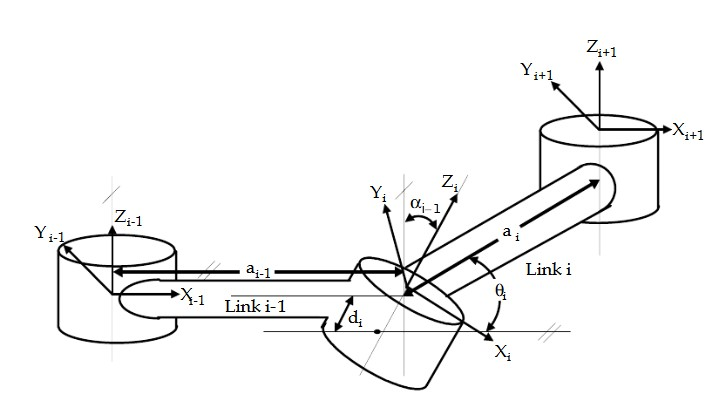
\includegraphics[width=0.9\textwidth]{figures/Coordinate frame assignment for a general manipulator.jpg}
\caption{順向運動學示例圖}
\end{figure}

如上圖所示,沿$X_{i-1}$測得的$Z_{i-1}$到$Z_{i}$的距離記$a_{i-1}$,沿$X_{i}$測得的$Z_{i-1}$和$Z_{i}$之間的角度為$\alpha_{i-1}$,沿$Z_{i}$測得的$X_{i-1}$到$X_{i}$的距離記$d_{i}$,沿$Z_{i}$測得的$X_{i-1}$到$X_{i}$的角度記$\theta_{i}$。\\
如此可求得變換矩陣${ }_{\mathrm{i}}^{\mathrm{i}-1} \mathrm{~T}$:

\small{
\begin{align}
\nonumber
& { }_{\mathrm{i}}^{\mathrm{i}-1} \mathrm{~T}=\mathrm{R}_{\mathrm{x}}\left(\alpha_{\mathrm{i}-1}\right) \mathrm{D}_{\mathrm{x}}\left(\mathrm{a}_{\mathrm{i}-1}\right) \mathrm{R}_{\mathrm{z}}\left(\theta_{\mathrm{i}}\right) \mathrm{Q}_{\mathrm{i}}\left(\mathrm{d}_{\mathrm{i}}\right) \\
\nonumber
& =
\left[\begin{array}{cccc}
1 & 0 & 0 & 0 \\
0 & \cos \alpha_{i-1} & -\sin \alpha_{i-1} & 0 \\
0 & \sin \alpha_{i-1} & \cos \alpha_{i-1} & 0 \\
0 & 0 & 0 & 1
\end{array}\right]
\nonumber
\left[\begin{array}{cccc}
1 & 0 & 0 & a_{i-1} \\
0 & 1 & 0 & 0 \\
0 & 0 & 1 & 0 \\
0 & 0 & 0 & 1
\end{array}\right]
\nonumber
\left[\begin{array}{cccc}
\cos \theta_{i} & -\sin \theta_{i} & 0 & 0 \\
\sin \theta_{i} & -\cos \theta_{i} & 0 & 0 \\
0 & 0 & 1 & 0\\
0 & 0 & 0 & 1
\end{array}\right]
\nonumber
\left[\begin{array}{cccc}
1 & 0 & 0 & 0 \\
0 & 1 & 0 & 0 \\
0 & 0 & 1 & d_{i} \\
0 & 0 & 0 & 1
\end{array}\right]\\
\nonumber
& =\left[\begin{array}{cccc}
\cos \theta_{i} & -\sin \theta_{i} & 0 & a_{i-1} \\
\sin \theta_{i} \cos \alpha_{i-1} & \cos \theta_{i} \cos \alpha_{i-1} & -\sin \alpha_{i-1} & -\sin \alpha_{i-1} d_{i} \\
\sin \theta_{i} \sin \alpha_{i-1} & \cos \theta_{i} \sin \alpha_{i-1} & \cos \alpha_{i-1} & \cos \alpha_{i-1} d_{i} \\
0 & 0 & 0 & 1
\end{array}\right] \\
\nonumber
&\end{align}}

而逆向運動學問題,實驗中使用了幾何求解(Geometric solution approach),與策略梯度方法(Policy-Gradient solution approach)~\cite{dauce2010inverse}來開發機械臂的逆向控制。\\

幾何求解方法的原理是將機械手臂的空間幾何問題分解為多個平面幾何問題,適用於機械結構較為簡單的機器人,如下圖所示:

\begin{figure}[htbp]
    \centering
    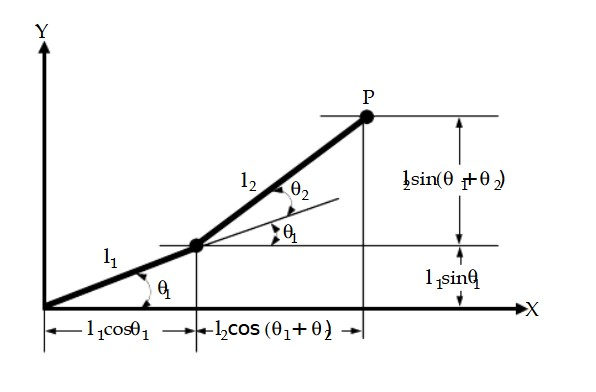
\includegraphics[width=0.9\textwidth]{figures/IK.jpg}
\caption{幾何求解逆向運動學示例圖}
\end{figure}

可由以下算式機算頂點$P$的分量($P_{x}$, $P_{y}$)。
$$
\begin{aligned}
& p_{x}=l_1 \cos \theta_1+l_2 \cos \theta_{12} \\
& p_{y}=l_1 \sin \theta_1+l_2 \sin \theta_{12}
\end{aligned}
$$
由於,$\cos \theta_{12}=\cos \theta_{1} \cos \theta_{2}-\sin \theta_{1} \sin \theta_{2}$,$
\sin \theta_{12}=\sin \theta_{1} \cos \theta_{2}-\cos \theta_{1} \sin \theta_{2}$,所以可得:

$$
\begin{aligned}
& p_{x}^2=l_1^2 \cos^2 \theta_1+l_2^2 \cos^2 \theta_{12}+2 l_1 l_2 \cos \theta_1 \cos \theta_{12} \\
& p_{y}^2=l_1^2 \sin^2 \theta_1 + l_2^2 \sin^2 \theta_{12}+2 l1_2 \sin \theta_1 \sin \theta_{12} \\
& p_{x}^2+p_{y}^2=l_1^2\left(\cos^2 \theta_1+\sin^2 \theta_1\right)+l_2^2\left(\cos^2 \theta_{12}+\sin^2 \theta_{12}\right)+2l_1 l_2\left(\cos \theta_1 \cos \theta_{12}+\sin \theta_1 \sin \theta_{12}\right)
\end{aligned}
$$

由於$\cos^2 \theta_{i}+\sin^2 \theta_{i}=1$,故可將上式化簡為:

$$
\begin{aligned}
& p_{x}^2+p_{y}^2=l_1^2+l_2^2+2l_1 l_2\left(c \theta_1\left[\cos \theta_1 \cos \theta_2-\sin \theta_1 \sin \theta_2\right]+\sin \theta_1\left[\sin \theta_1 \cos \theta_2+\cos \theta_1 \sin \theta_2\right]\right) \\
& p_{x}^2+p_y^2=l_1^2+l_2^2+2l_1 l_2\left(\cos^2 \theta_1 \cos \theta_2-\cos \theta_1 \sin \theta_1 \sin \theta_2+\sin^2 \theta_1 \cos \theta_2+\cos \theta_1 \sin \theta_1 \sin \theta_2\right) \\
& p_{x}^2+p_y^2=l_1^2+l_2^2+2l_1 l_2\left(\cos \theta_2\left[\cos^2 \theta_1+\sin^2 \theta_1\right]\right) \\
& p_{x}^2+p_{y}^2=l_1^2+l_2^2+2l_1 l_2 \cos \theta_2
\end{aligned}
$$

由移項後得:

$$
\begin{aligned}
& \cos \theta_2=\frac{p_{x}^2+p_{y}^2-l_1^2-l_2^2}{2l_1 l_2} \\
& \sin \theta_2= \pm \sqrt{1-\left(\frac{p_{x}^2+p_{y}^2-l_1^2-l_2^2}{2l_1 l_2}\right)^2} \\
& \theta_2=A \tan 2\left( \pm \sqrt{1-\left(\frac{p_{x}^2+p_{y}^2-l_1^2-l_2^2}{2l_1 l_2}\right)^2}, \frac{p_{x}^2+p_{y}^2-l_1^2-l_2^2}{2l_1 l_2}\right)
\end{aligned}
$$

繼續利用$\theta_2$求解$\theta_1$:
將$p_{x}=l_1 \cos \theta_1+l_2 \cos \theta_{12}$等號兩邊同乘$\cos \theta_1$
將$p_{y}=l_1 \sin \theta_1+l_2 \sin \theta_{12}$等號兩邊同乘$\sin \theta_1$得:
$$
\begin{aligned}
& \cos \theta_1 p_{x}=l_1 \cos^2 \theta_1+l_2 \cos^2 \theta_1 \cos \theta_2-l_2 \cos \theta_1 \sin \theta_1 \sin \theta_2 \\
& \sin p_{y}=l_1 \sin^2 \theta_1+l_2 \sin^2 \theta_{1} \cos \theta_2+l_2 \sin \theta_1 \cos \theta_1 \sin \theta_2 \\
& \cos \theta_1 p_{x}+\sin \theta_1 p_{y}=l_1\left(\cos^2 \theta_1+\sin^2 \theta_1\right)+l_2 \theta_2\left(\cos \theta_1+\sin^2 \theta_1\right)
\end{aligned}
$$
可化簡為:
$$
& \cos \theta_1 p_{x}+\sin \theta_1 p_{y}=l_1+l_2 \cos \theta_2
$$

將$p_{x}=l_1 \cos \theta_1+l_2 \cos \theta_{12}$等號兩邊同乘$-\sin \theta_1$
將$p_{y}=l_1 \sin \theta_1+l_2 \sin \theta_{12}$等號兩邊同乘$\cos \theta_1$得:
$$
\begin{aligned}
& -\sin \theta_1 p_{x}=-l_1 \sin \theta_1 \cos \theta_1-l_2 \sin \theta_1 \cos \theta_1 \cos \theta_2+l_1 \sin^2 \theta_1 \sin \theta_2 \\
& \cos \theta_1 p_{y}=l_1 \sin \theta_1 \cos \theta_1+l_2 \cos \theta_1 \sin \theta_1 \cos \theta_2+l_2 \cos^2 \theta_1 \sin \theta_2 \\
& -\sin \theta_1 p_{x}+\cos \theta_1 p_{y}=l_2 \sin \theta_2\left(\cos^2 \theta_1+\sin \theta_1\right)
\end{aligned}
$$
可化簡為:
$$
& -\sin \theta_1 p_{x} + \cos \theta_1 p_{y} = l_2 \sin \theta_2
$$

最後,將$\cos \theta_1 p_{x}+\sin \theta_1 p_{y}=l_1+l_2 \cos \theta_2$等號兩邊同乘$P_x$,$-\sin \theta_1 p_{x} + \cos \theta_1 p_{y} = l_2 \sin \theta_2$等號兩邊同乘$P_y$,得:

$$
\begin{aligned}
& \cos \theta_1 p_{x}^2 + \sin \theta_1 p_x p_y = p_x \left(l_1 + l_2 \cos \theta_2 \right) \\
& - \sin \theta_1 p_x p_y + \cos \theta_1 p_{y}^2 = p_y l_2 \sin \theta_2 \\
& \cos \left(p_{x}^2+p_{y}^2 \right) = p_x \left(l_1+l_2 \cos \theta_2 \right) _ p_y l_2 \sin \theta_2
\end{aligned}
$$
可求出$\theta_1$:
$$
\begin{aligned}
& \cos \theta_1= \frac{p_{x} \left{l_1+l_2 \cos \theta_2 \right}+p_y l_2 \sin \theta_2}{p_{x}^2 + p_{y}^2}
& \sin \theta_1= \pm \sqrt{1-\left(\frac{p_{x} \left{l_1 + l_2 \cos \theta_2 \right}+p_y l_2 \sin \theta_2}{p_x^2 = p_y^2}\right)^2}
& \theta_1=A \tan 2\left( \pm \sqrt{1-\left(\frac{p_{x}\left(l_1+l_2 \cos \theta_2\right)+p_{y} l_2 \sin \theta_2}{p_{x}^2+p_{y}^2}\right)^2}, \frac{p_{x}\left(l_1+l_2 \cos \theta_2\right)+p_{y} l_2 \sin \theta_2}{p_{x}^2+p_{y}^2}\right)
\end{aligned}
$$

以上為使用幾何求解逆向運動學的簡易範例,可以看出使用此方法求解需要繁瑣的計算。 \\

以下介紹使用策略梯度方法求解逆向運動學的計算方式:

\subsection{3D列印應用於機器人製作的相關文獻}
引用carbon design的相關論文並進一步討論(用於設計3D模型)

\end{document}    % 背景知識及文獻回顧
        \documentclass[class=NCU_thesis, crop=false]{standalone}
\begin{document}

\chapter{研究方法}
\section{硬體設計流程}
\subsection{模型設計軟體:Autodesk Fusion 360}
Autodesk Fusion 360是一款集合了電腦輔助設計(Computer-Aided Design, CAD)、電腦輔助製造(Computer-Aided Manufacturing, CAM)、電腦輔助工程(Computer-Aided Engineering, CAE)及印刷電路板設計(Printed Circuit Board, PCB)的多功能設計軟體。由於結合了眾多工具,所以在產品設計、工程設計、機械設計和製造等眾多領域都累積了一定規模的使用者,也成為許多設計師、工程師和製造專業人士的首選工具。

\begin{itemize}
	\item 3D建模:提供精準的參數化建模,方便使用者精準的設計每一個零件的細節。
	\item 裝配設計:模擬多個零件組合後的裝配設計,能確認組合後的零件是否能正常運作。
	\item 渲染與設計圖生成:內建強大的渲染引擎,可以生成高質量的圖像和客製化設計圖,以便更好的展示設計成果。
	\item 模型庫:官方與使用者社群建立的廣大模型庫,能找到市面上多數的電路板、馬達與零件模型,方便使用者將這些零件一起納入設計圖。
	\item 雲端協作:Autodesk擁有自己的雲端平台,團隊成員可以實時共享和協作設計,方便遠端工作和版本控制。
\end{itemize}

\begin{figure}[htbp]
    \centering
    
\includegraphics[width=0.9\textwidth]{figures/autodesk-fusion-360-seeklogo.png}
\caption{Autodesk Fusion 360 Logo}
\end{figure}

\subsection{檔案輸出格式:STL(Stereolithography)}
STL(Stereolithography)是一種常用的3D模型文件格式,特別是在3D列印領域中廣泛應用。STL格式最早由3D Systems公司在1987年為其立體光刻(SLA)3D列印技術開發,但隨後成為各類3D列印技術的標準文件格式。STL文件描述了3D物體的表面幾何形狀,不包含任何顏色、材質或其他屬性。以下為使用STL格式用於3D列印的優勢:

\begin{itemize}
	\item 簡單性:STL格式結構簡單,易於生成和處理。
	\item 廣泛性:幾乎所有的3D建模和3D列印軟體都支援STL檔案格式。
	\item 精度彈性:可以通過調整三角形數量來控制模型的精度和細節,適應不同的列印需求。
	\item 輕量:STL格式僅描述幾何形狀,不包含顏色、材質或其他屬性資訊,正好符合3D列印只需幾何形狀的需求。
\end{itemize}

\begin{figure}[htbp]
    \centering
    
\includegraphics[width=0.9\textwidth]{figures/3D_Systems_Logo.png}
\caption{3D Systems Logo}
\end{figure}

\subsection{3D列印機:Creality K1 MAX}
本實驗選擇使用的3D列印機為Creality K1 MAX,以下為該機型的主要特點:
\begin{itemize}
	\item 大尺寸打印:使用CoreXY運動結構,高達300x300x300mm的列印面積,能夠滿足大型模型的列印需求。
	\item 解析度:具有極高的打印解析度,可以實現細膩的表面細節和精確的尺寸控制。
	\item 高速列印:配備了高效的運動系統和強大的驅動機構,最高能達到600mm/s的高速列印、20000mm/s²的加速度與32mm³/s 的超大流量,能夠顯著縮短列印時間。
	\item 耗材多樣性:支援多種列印耗材,包括PLA、ABS、TPU等,為使用者提供了更多創作自由度。
\end{itemize}

\begin{figure}[htbp]
    \centering
    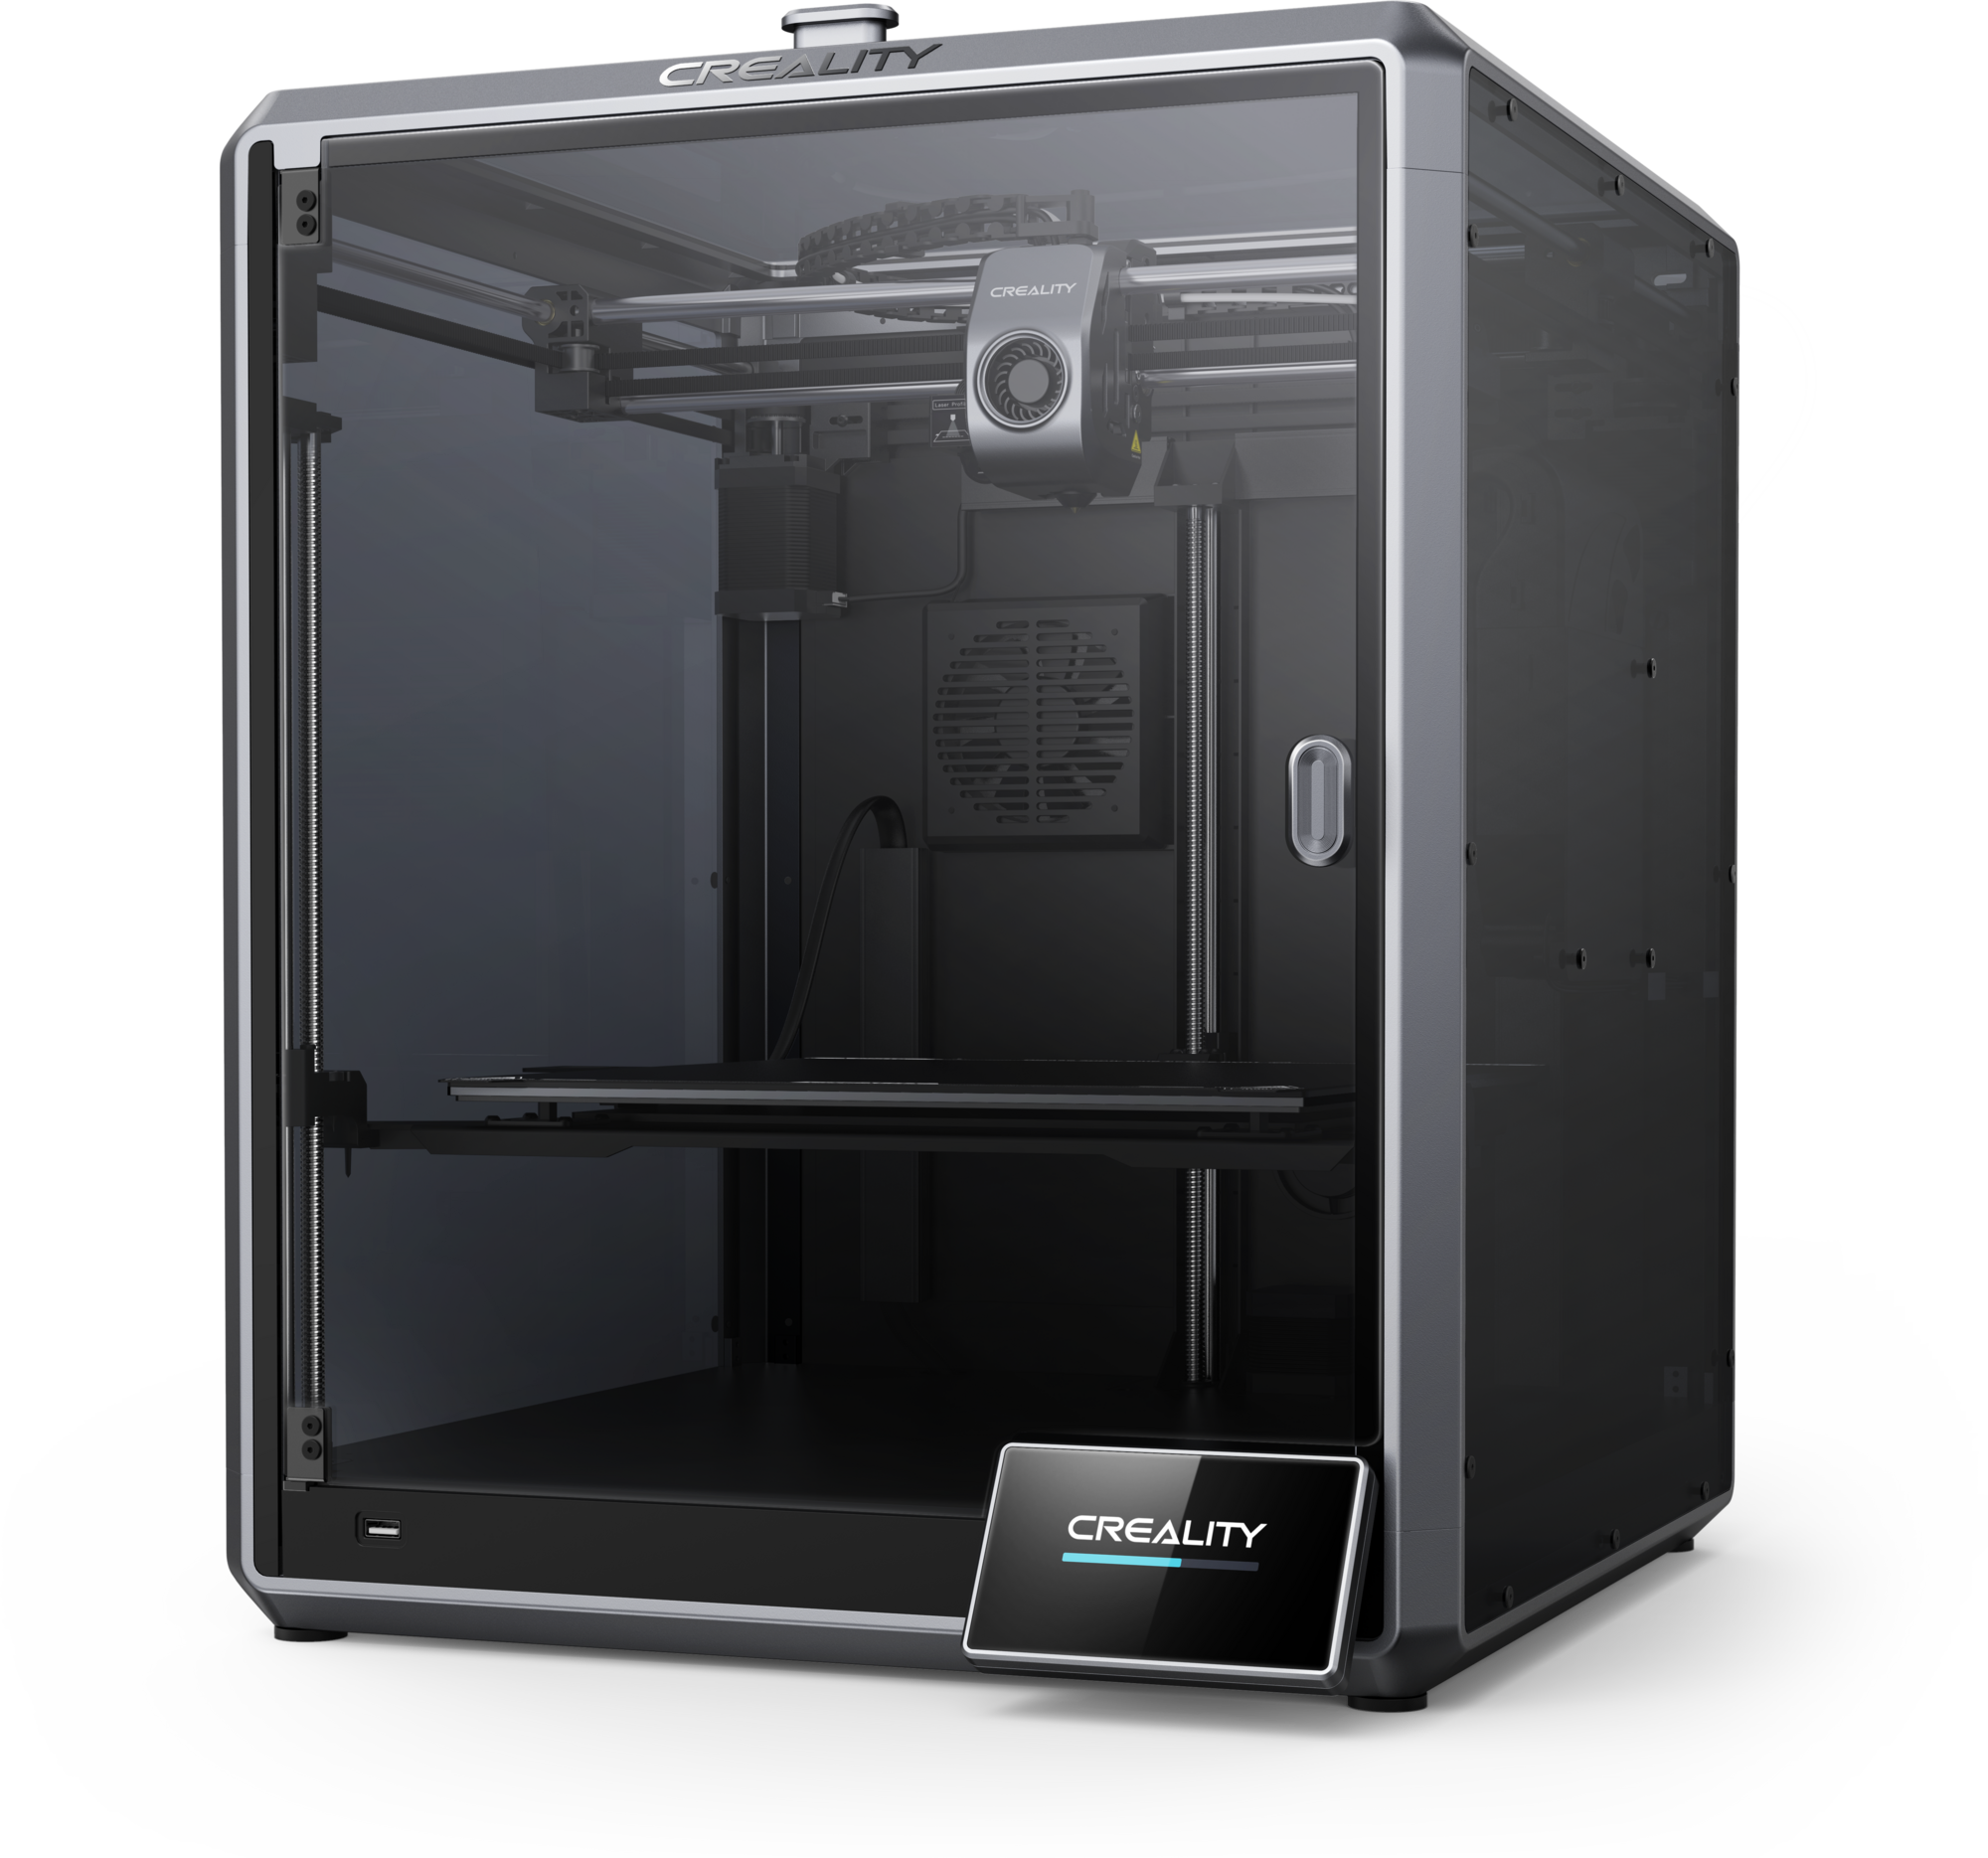
\includegraphics[width=0.9\textwidth]{figures/creality-k1-max.png}
\caption{Creality K1 MAX}
\end{figure}

\subsection{馬達與開發版介紹}
以下為本論文使用到的零件簡介:

1. SG90,是一款微型伺服馬達,由於扭矩較小,所以本實驗將其用於機械臂後段(頂點)。它的特點包括:
\begin{itemize}
	\item 重量:小巧輕便,重量僅為9克。
	\item 操作電壓:4.8V至6.0V。
	\item 扭矩:在4.8V時可達1.8kg/cm。
	\item 控制方式:使用PWM信號來控制轉角,通常範圍為0°至180°。
\end{itemize}

2. MG90S,是一款金屬齒輪伺服馬達,由於扭矩適中,所以本實驗將其用於機械臂前中段。其特點包括:
\begin{itemize}
	\item 重量:重量約為14g,稍大於SG90,但仍屬於微型伺服馬達。
	\item 操作電壓:4.8V至6.0V。
	\item 扭矩:在4.8V時可達2.2kg/cm。
	\item 控制方式:使用PWM信號來控制轉角,通常範圍為0°至180°。
\end{itemize}

3. MG996R,是一款高扭矩伺服馬達,由於扭矩較大,所以本實驗將其用於機械臂前段。其主要特點包括:
\begin{itemize}
	\item 尺寸:重量約為55g,適用於中型或大型專案。
	\item 操作電壓:4.8V至7.2V。
	\item 扭矩:在6.0V時可達9.4kg/cm。
	\item 控制方式:使用PWM信號來控制轉角,通常範圍為0°至180°。
\end{itemize}

4. Raspberry Pi 4,是一款高性能的嵌入式裝置。其主要特點包括:
\begin{itemize}
	\item 處理器:四核ARM Cortex-A72,1.5GHz。
	\item 內存:有2GB、4GB和8GB可選,本實驗採用8GB內存。
	\item 輸入/輸出:支援USB 3.0、HDMI、GPIO、以太網等連接方式,同時也支援wifi藍芽等無線連接方式
	\item 作業系統:本實驗採用Raspberry Pi OS(基於Debian)。
\end{itemize}

5. ESP32-S3-Devkit,是一款高性能、低功耗的微控制器,適合用於物聯網應用。其主要特點包括:
\begin{itemize}
	\item 處理器:雙核Xtensa LX7,最高240MHz。
	\item 內存:512KB SRAM,支持外部RAM擴展。
	\item 輸入/輸出:支援microUSB連接方式,同時也支援Wi-Fi和藍芽等無線連接方式。
	\item 作業系統:本實驗採用circuit python。
\end{itemize}

6. ESP32 Doit-Devkit,是一個常見的ESP32開發板,設計簡單且功能強大。其主要特點包括:
\begin{itemize}
	\item 處理器:雙核Xtensa LX6,最高240MHz。
	\item 內存:520KB SRAM。
	\item 支援microUSB連接方式,同時也支援Wi-Fi和藍芽等無線連接方式。
	\item 作業系統:本實驗採用circuit python。
\end{itemize}

7. L298N,直流馬達驅動模組,常用於控制雙馬達系統,本實驗將此裝置用於控制車輪。其主要特點包括:
\begin{itemize}
	\item 電壓範圍:可操作電壓範圍為5V至35V。
	\item 電流:每通道峰值電流可達2A。
	\item 控制:使用PWM訊號控制馬達速度和方向。
\end{itemize}

8. PCA9685,是一款16通道PWM驅動模組,通常用於控制伺服馬達和LED燈,本實驗將此裝置用於控制機械臂馬達。其主要特點包括:
\begin{itemize}
	\item PWM頻率:可調頻率範圍為24Hz至1526Hz。
	\item 接口:使用I2C介面進行訊號傳輸。
	\item 控制:使用PWM訊號控制馬達速度和方向,適合需要一次性控制大量馬達的專案。
\end{itemize}

\begin{figure}[!hbt]
    \centering
    \subcaptionbox
        {SG90
        \label{fig:fig-dataset-contrast-after-adjustment}}
        {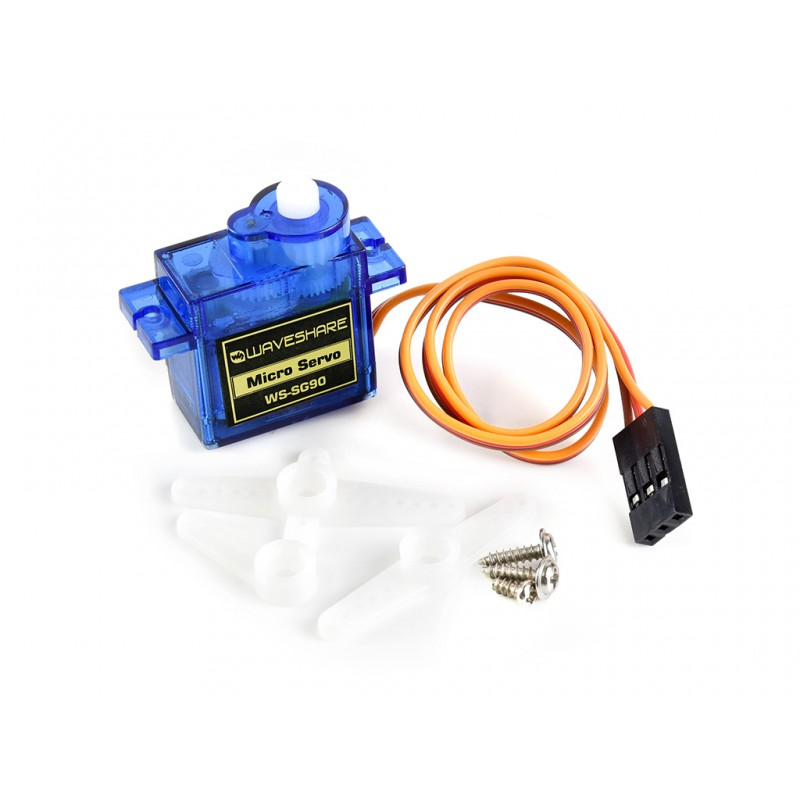
\includegraphics[width=0.25\linewidth]{figures/SG90.jpg}}
    ~    
    \subcaptionbox
        {MG90S
        \label{fig:fig-dataset-contrast-after-adjustment}}
        {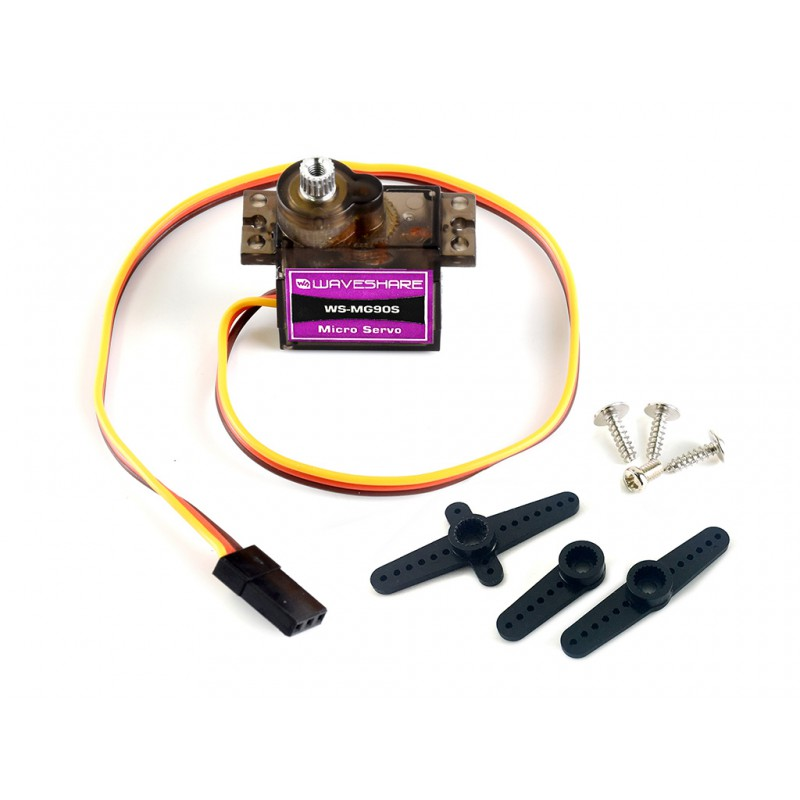
\includegraphics[width=0.25\linewidth]{figures/MG90S.jpg}}
    ~    
    \subcaptionbox
        {MG996R
        \label{fig:fig-dataset-contrast-after-adjustment}}
        {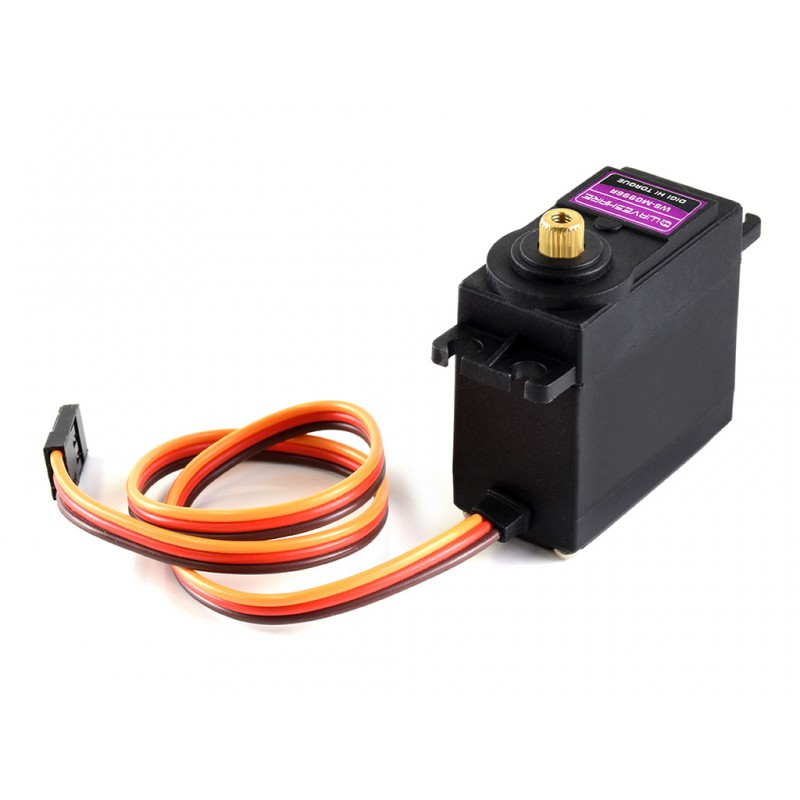
\includegraphics[width=0.25\linewidth]{figures/MG996R.jpg}}
    ~   
    \subcaptionbox
        {Raspberry Pi 4
        \label{fig:fig-dataset-contrast-after-adjustment}}
        {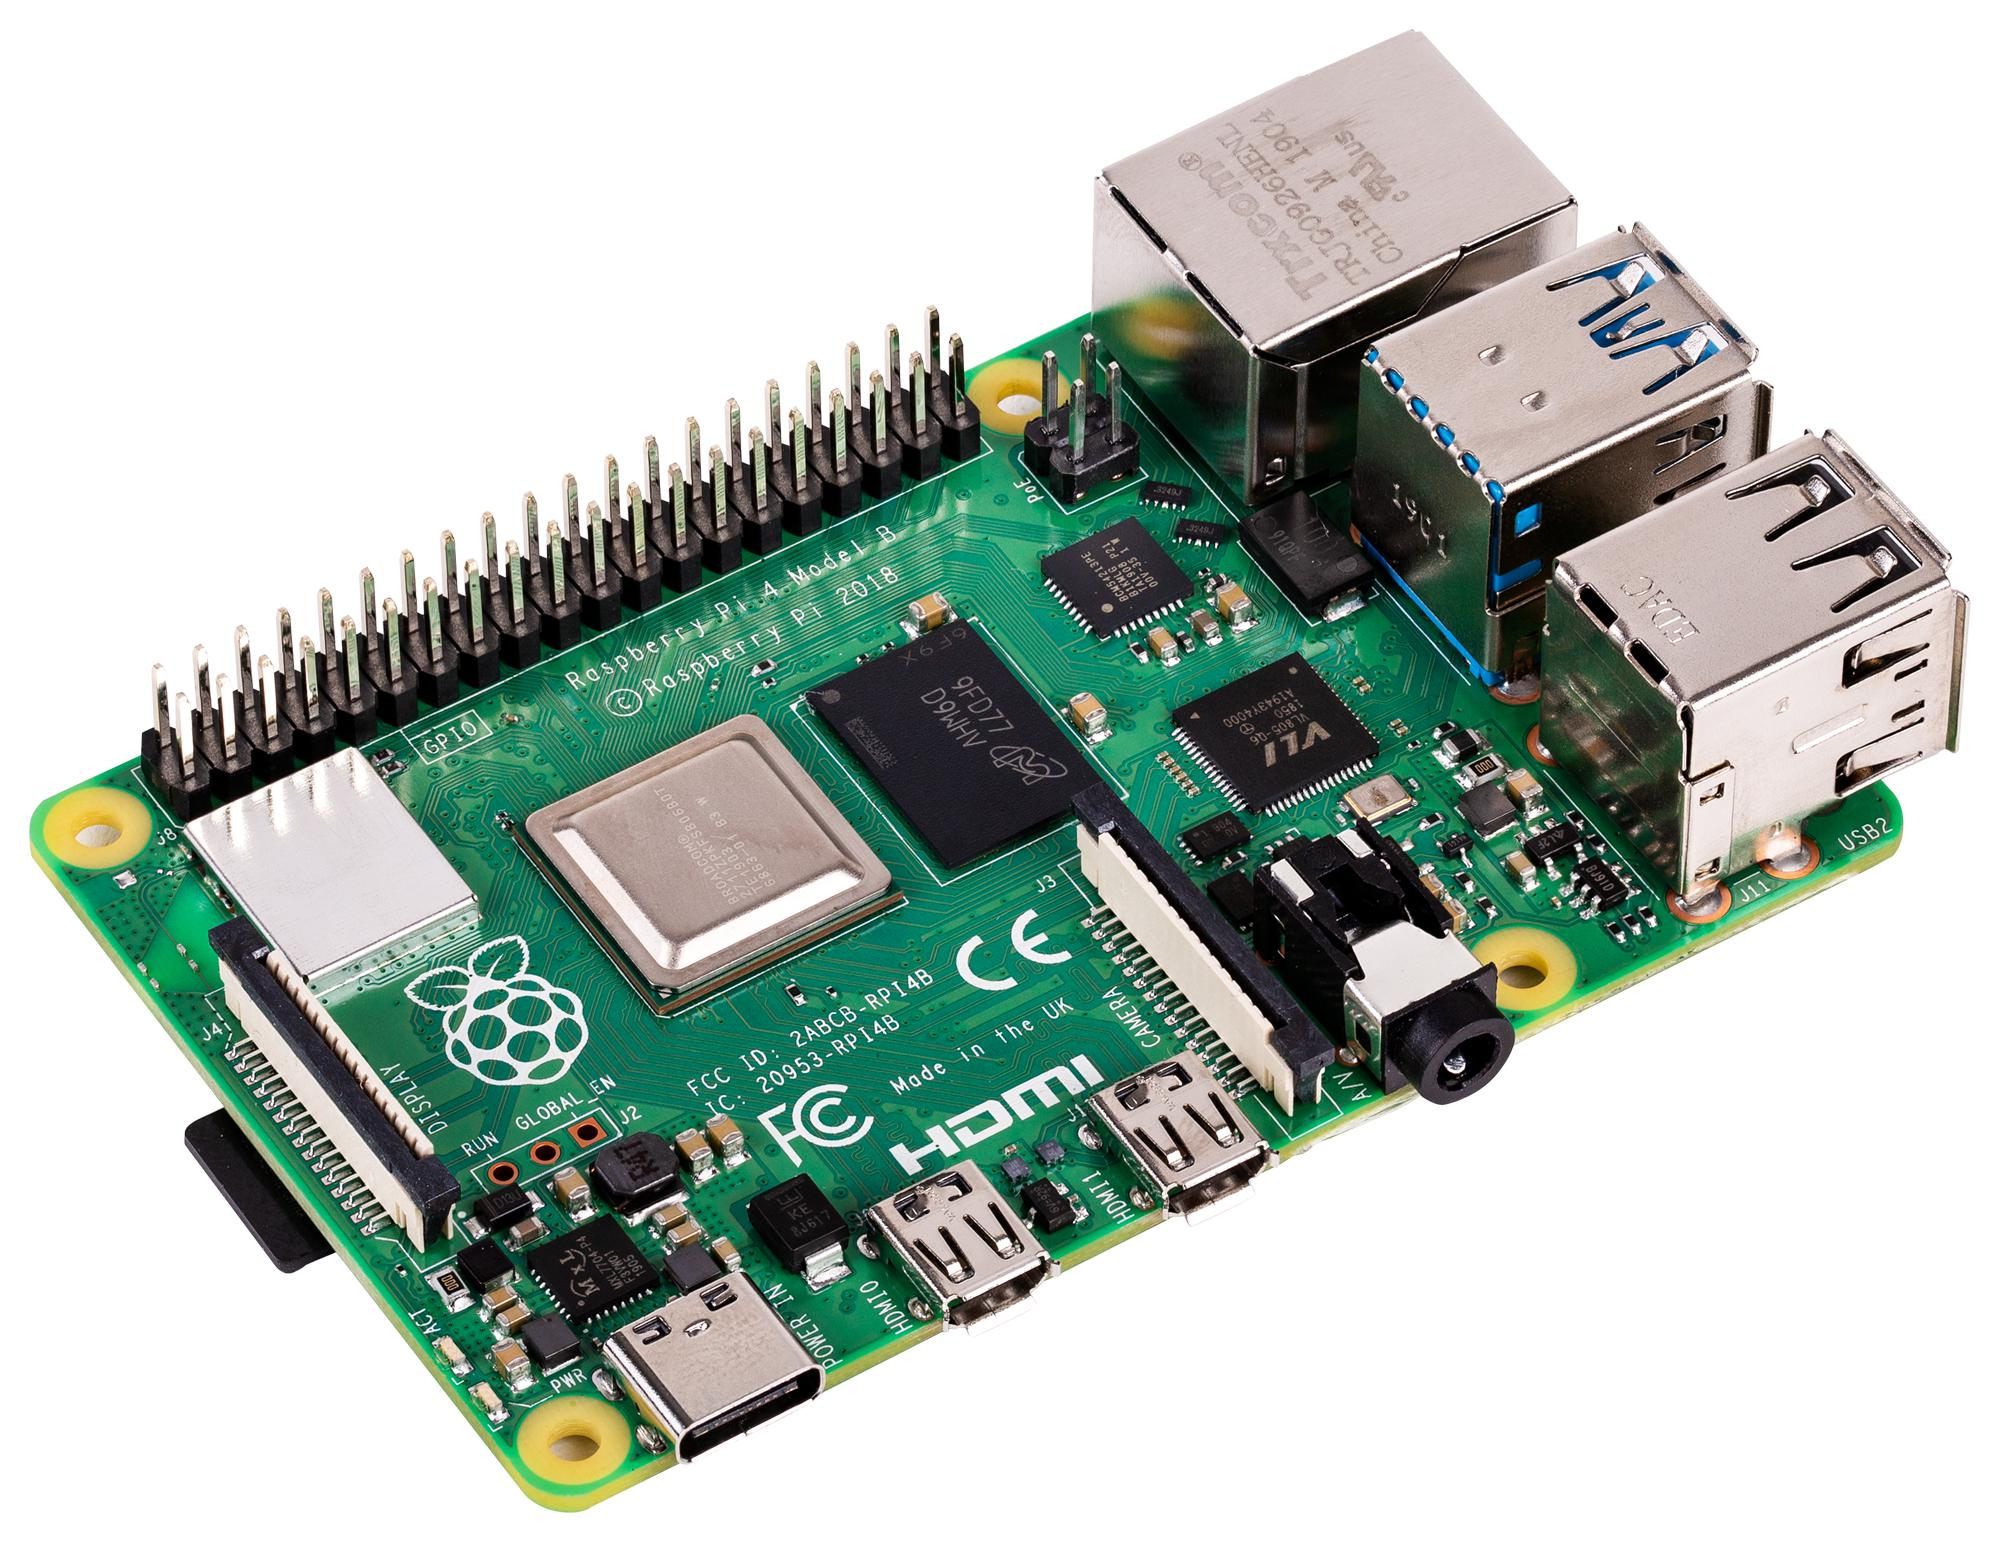
\includegraphics[width=0.25\linewidth]{figures/Rasberry pi 4.jpg}}
    ~    
    \subcaptionbox
        {ESP32-S3-Devkit
        \label{fig:fig-dataset-contrast-after-adjustment}}
        {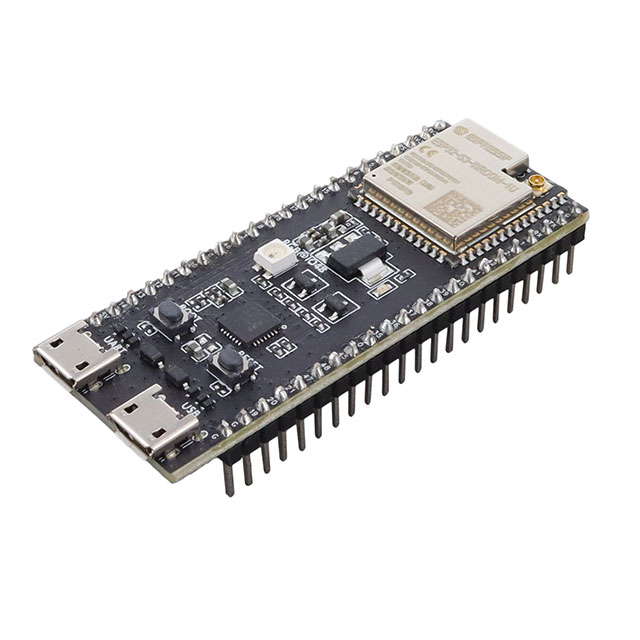
\includegraphics[width=0.25\linewidth]{figures/ESP32-S3.jpg}}
    ~    
    \subcaptionbox
        {ESP32 Doit-Devkit
        \label{fig:fig-dataset-contrast-after-adjustment}}
        {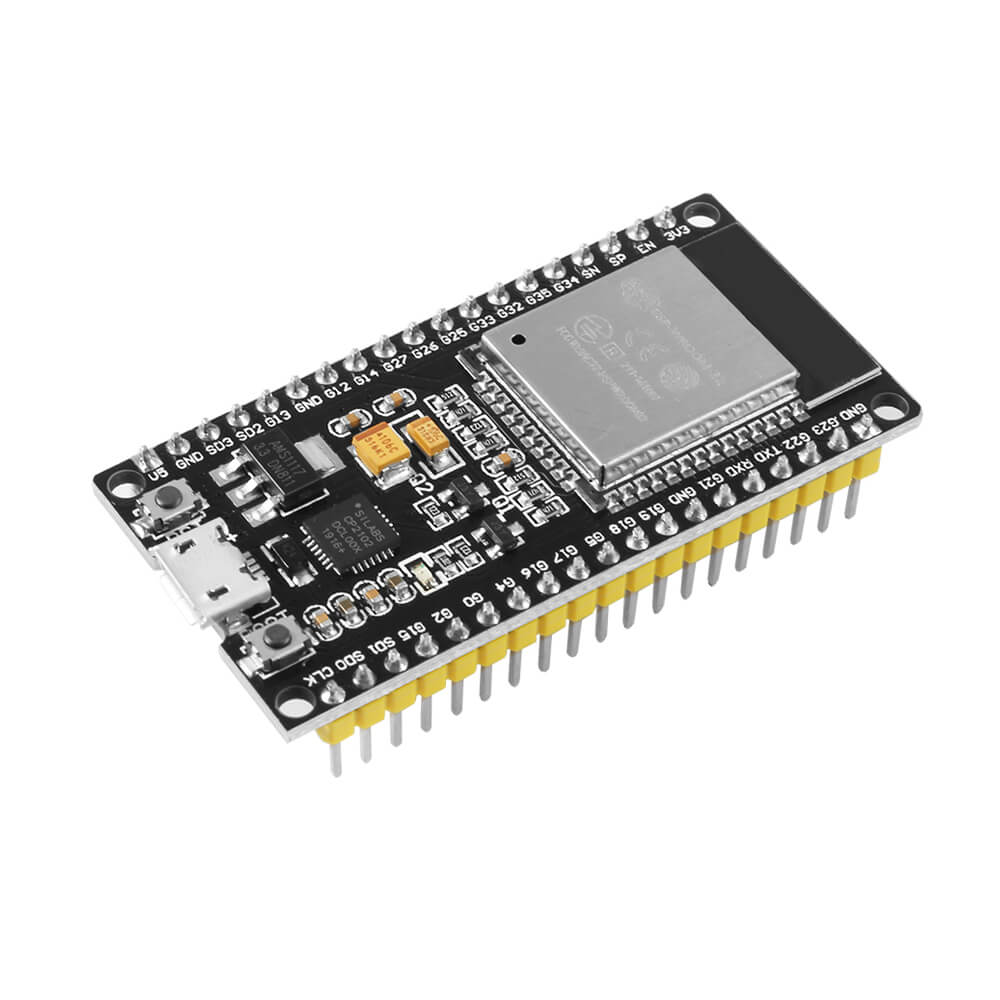
\includegraphics[width=0.25\linewidth]{figures/ESP32-DOIT.jpg}}
    ~  
    \subcaptionbox
        {L298N
        \label{fig:fig-dataset-contrast-after-adjustment}}
        {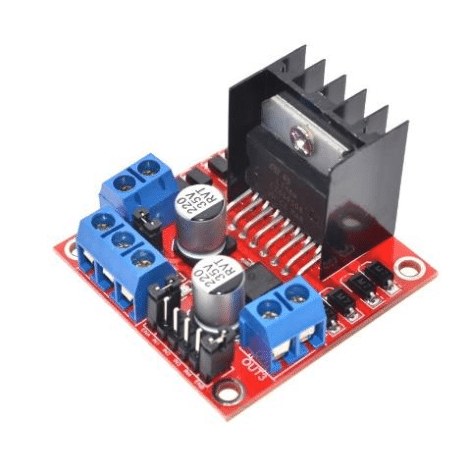
\includegraphics[width=0.25\linewidth]{figures/L298N.png}}
    ~    
    \subcaptionbox
        {PCA9685
        \label{fig:fig-dataset-contrast-after-adjustment}}
        {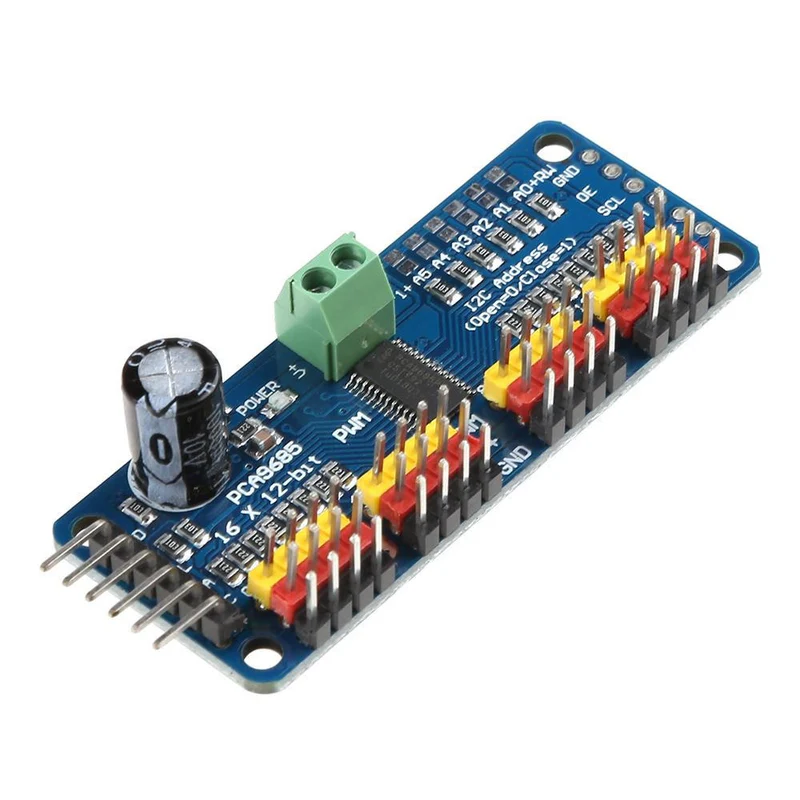
\includegraphics[width=0.25\linewidth]{figures/PCA9685.png}}
\caption{實驗一:實驗過程縮圖}
\end{figure}

\section{運動學開發}

\subsection{運動模擬環境}
本專案使用Python語言開發了一個簡易的機械臂模擬環境。這個模擬環境的基本原理,是將機械臂定義為一個擁有多個可調整參數的獨立物件,其中包括力臂長度、扭轉角、節點偏移、節點角度、目標頂點、和目前頂點等。這些參數可以由使用者根據需求進行調整,從而在虛擬空間中生成機械臂的模型。該模擬環境提供了一個直觀且靈活的介面,使得使用者能夠方便地設計和測試機械臂的運動行為。

\begin{listing}
    \begin{minted}[frame=single,
                   framesep=3mm,
                   linenos=true,
                   xleftmargin=21pt,
                   tabsize=4]{python}

        class ArmEnv_3D:
            def __init__(self, lList, vision=True):
                self.Link_length = lList
                self.Link_offset=[0]*len(lList)
                self.Twist_angle=[0]*len(lList)
                self.Joint_angle = [0]*len(lList)
                self.Target_point=[0, 0, 0]
                self.Current_point=[0, 0, sum(lList)]

            def Forward_kinematics(self, joint_angles):...
            
            def Geometric_solution(self):...

            def Gradient_policy(self,times=100, points=10, speed=5):...

            def initPicture(self):...

            def updatePicture(self):...

    \end{minted}
\caption{運動模擬環境程式架構} 
\end{listing}

\subsection{順向運動學}
在順向運動學部分,本專案採用了Denavit-Hartenberg方法作為主要的計算方式。這種方法能夠系統地描述和計算機械臂的運動行為。模擬環境中的相關函式可以直接被呼叫,利用即時的機械臂參數來計算操作點的空間座標。計算結果會即時顯示在模擬空間中。

\subsection{逆向運動學}
在逆向運動學方面,本專案結合了幾何求解(Geometric solution approach)方法和策略梯度(Policy-Gradient solution approach)方法來進行計算。幾何求解方法主要用於計算運動模式較為簡單的機械臂,而策略梯度方法則適用於運動較為複雜的機械臂。這些計算函式同樣可以在模擬環境中直接被呼叫。根據輸入的目標操作點位置,系統會計算出對應的扭轉角,並將結果顯示在模擬空間中。

\section{大型語言模型選擇}
\subsection{open ai介紹}
\subsection{下prompt的規則}

\section{系統架構}
\subsection{系統架構圖}
整個系統架構介紹
\subsection{client端的輸入內容}
\subsection{轉換到code的過程}

\end{document}          % 研究方法
        \documentclass[class=NCU_thesis, crop=false]{standalone}
\usepackage[newfloat]{minted}
\usepackage{floatrow}
\usepackage{graphicx}


\begin{document}

\chapter{實驗設計與結果}

\section{實驗一:機械臂的基本控制}
\subsection{機械結構設計圖}
本實驗的硬體部分使用了3D列印技術,結合小型伺服馬達,設計了一個頂端為夾爪的小型機械臂,以下為此硬體的詳細設計圖紙:
\begin{figure}[htbp]
    \centering
    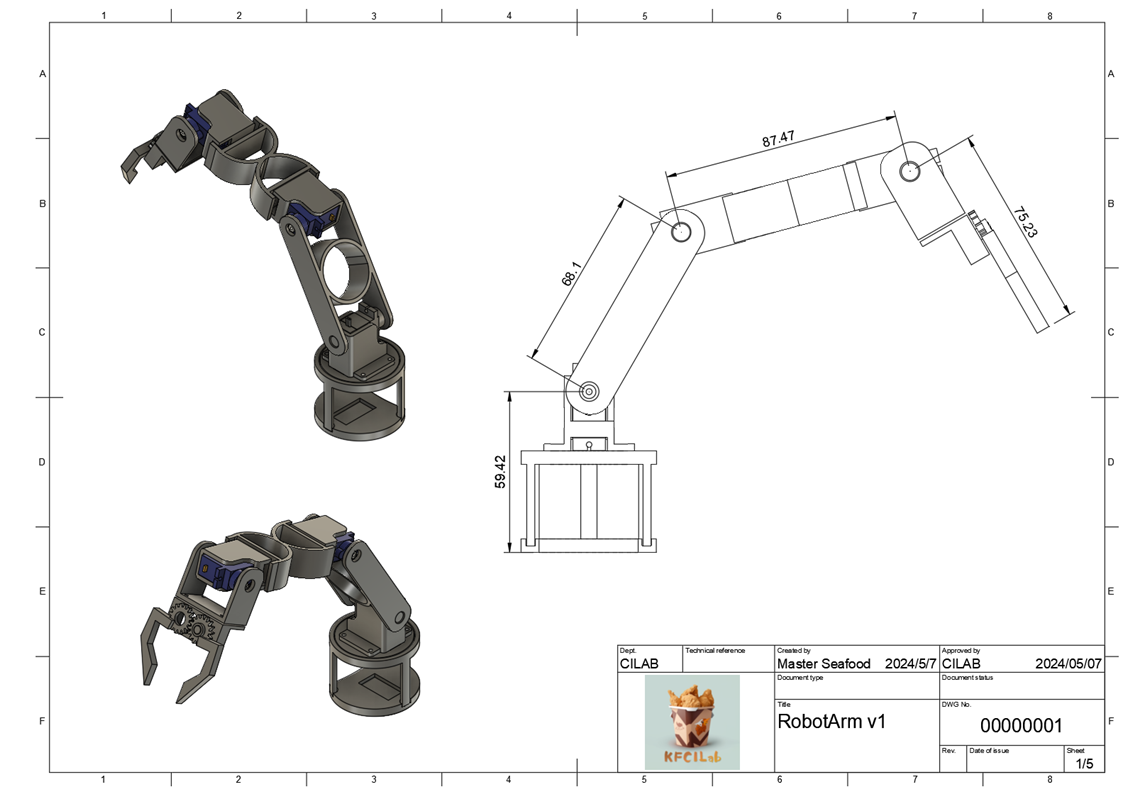
\includegraphics[width=0.9\textwidth]{figures/Armv1 (1).PNG}
    \caption{機械臂版本一設計圖紙 第一頁(單位:mm)}
    %\label{fig:Armv1Drawing_p1}}
\end{figure}

\begin{figure}[htbp]
    \centering
    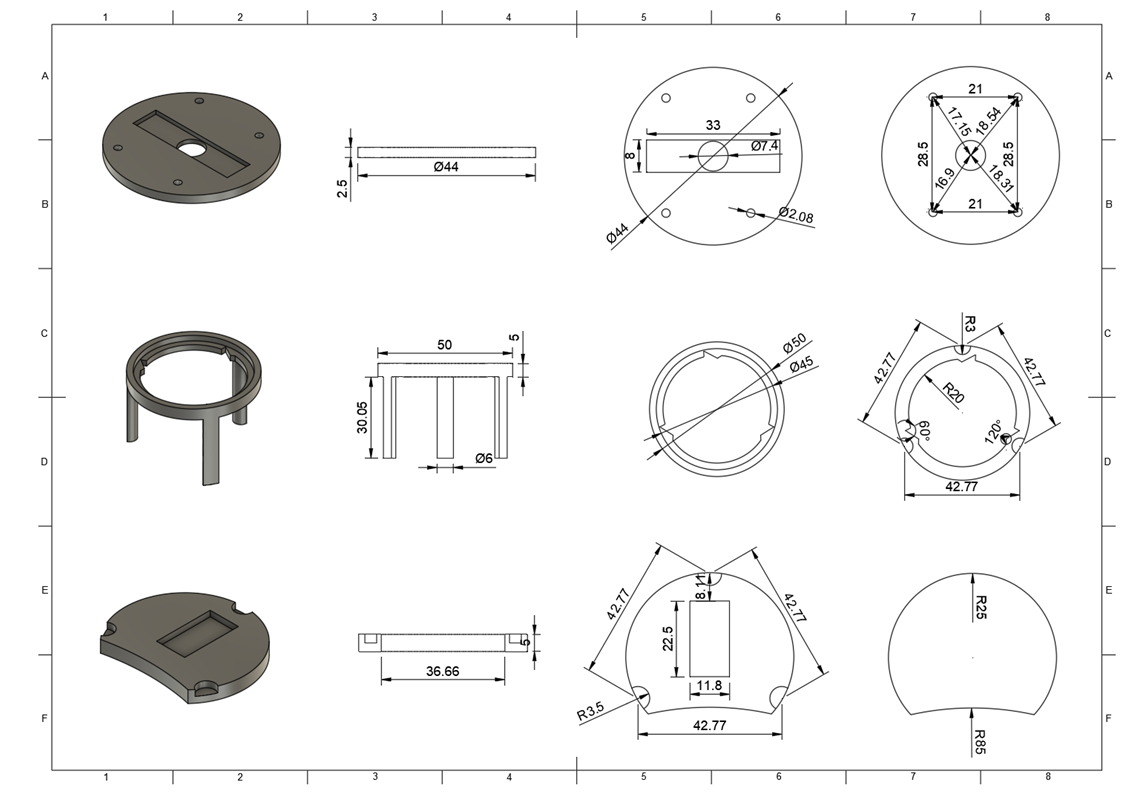
\includegraphics[width=0.9\textwidth]{figures/Armv1 (2).PNG}
    \caption{機械臂版本一設計圖紙 第二頁(單位:mm)}
\end{figure}

\begin{figure}[htbp]
    \centering
    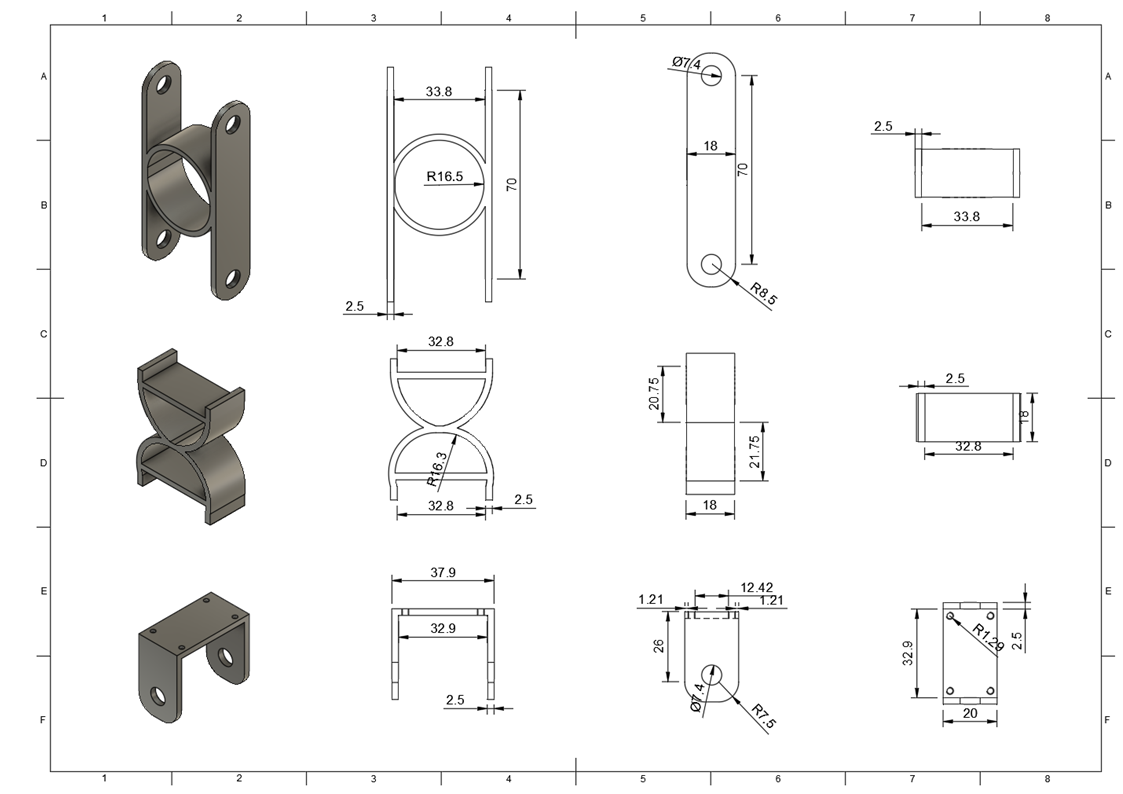
\includegraphics[width=0.9\textwidth]{figures/Armv1 (3).PNG}
    \caption{機械臂版本一設計圖紙 第三頁(單位:mm)}
\end{figure}

\begin{figure}[htbp]
    \centering
    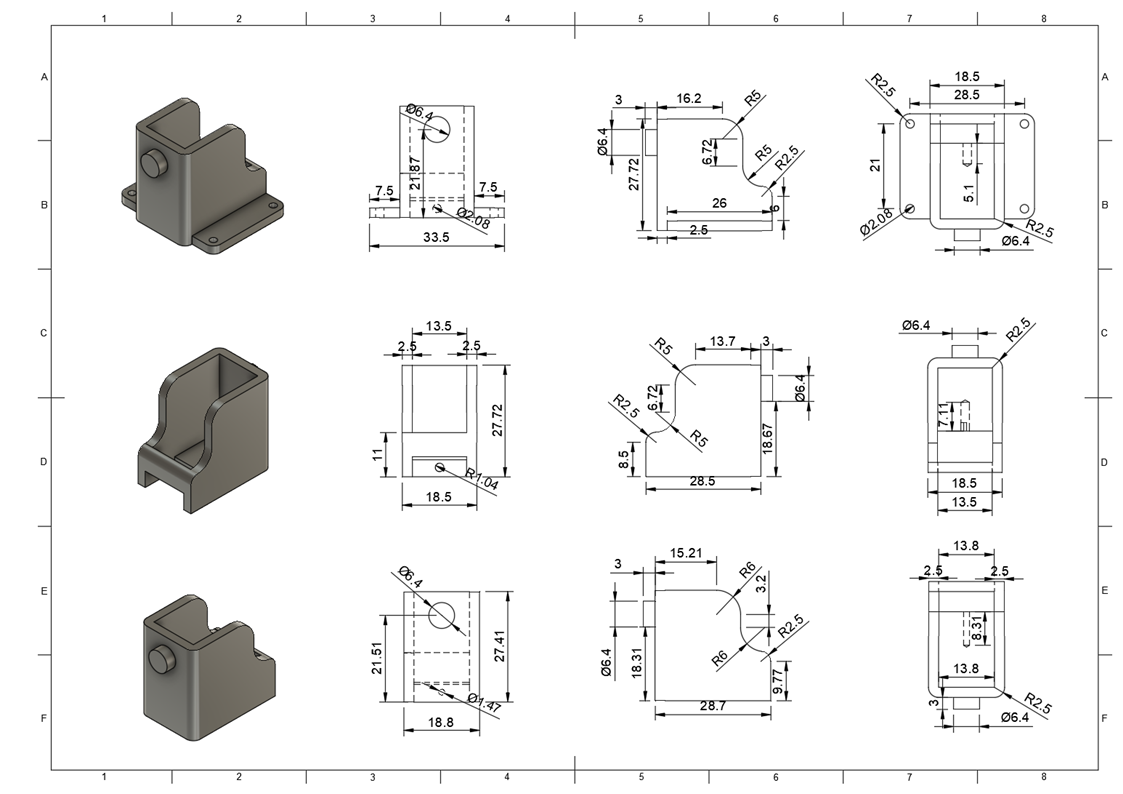
\includegraphics[width=0.9\textwidth]{figures/Armv1 (4).PNG}
    \caption{機械臂版本一設計圖紙 第四頁(單位:mm)}
\end{figure}

\begin{figure}[htbp]
    \centering
    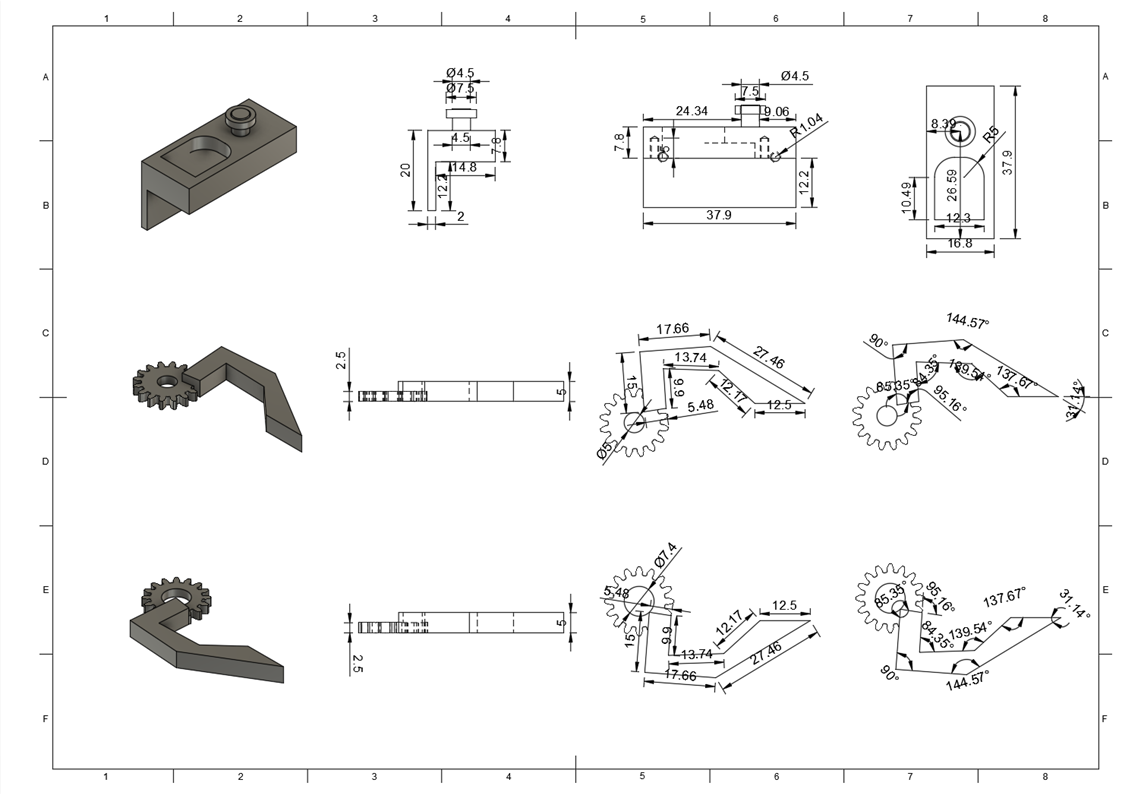
\includegraphics[width=0.9\textwidth]{figures/Armv1 (5).PNG}
    \caption{機械臂版本一設計圖紙 第五頁(單位:mm)}
\end{figure}

\subsection{函數設計}
在這個實驗中,我們的目標是讓機械臂能夠成功夾取特定物體,並放置於指定位置。
這個過程涉及機械臂路徑的規劃和精確的抓取動作。
為了實現這一目標,我們撰寫了一個簡易的路徑規劃程式,
利用語言模型在填空方面的優勢,使其生成和編輯機械臂的運動指令。
使用這樣的方式,嘗試讓大型語言模型自動生成適當的路徑規劃,並將其應用於機械臂的控制,
以下為此實驗使用的程式碼:\\
\begin{listing}[h]
    \begin{minted}[frame=single,
                   framesep=3mm,
                   linenos=true,
                   xleftmargin=21pt,
                   tabsize=4]{python}
        from ArmEnv_3D_ori import ArmEnv_3D
        import math

        Arm = ArmEnv_3D([5.942, 6.81, 8.747, 7.523], False)
        path = []
        #Please planning path form hear
        #path+=Arm.moveto([0, 0, 25], 20) explain: Move to [0, 0, 25] in 20 steps
        #path+=[[-91, 0, 0, 0]] explain: Close claw
        #path+=[[91, 0, 0, 0]] explain: Open claw

        #reset
        end=path[-2].copy()
        while not sum(end)==0:
            for i in range(len(end)):
                if end[i]>0: end[i]-=1
                elif end[i]<0: end[i]+=1
            path.append(end.copy())
    \end{minted}
\caption{實驗程式碼} 
\end{listing}
\clearpage

\subsection{下達指令的格式範例}
\begin{listing}[h]
    \begin{minted}[frame=single,
                   framesep=3mm,
                   linenos=true,
                   xleftmargin=21pt,
                   tabsize=4]{js}
    {     
        role: "user",
        content : 
    "\
    from ArmEnv_3D_ori import ArmEnv_3D\
    import math\
    \
    Arm = ArmEnv_3D([5.942, 6.81, 8.747, 7.523], False)\
    path = []\
    #Please planning path form hear\
    #path+=Arm.moveto([0, 0, 25], 20) explain: Move to [0, 0, 25] in 20 steps\
    #path+=[[-91, 0, 0, 0]] explain: Close claw\
    #path+=[[91, 0, 0, 0]] explain: Open claw\
    \
    #reset\
    end=path[-2].copy()\
    while not sum(end)==0:\
        for i in range(len(end)):\
            if end[i]>0: end[i]-=1\
            elif end[i]<0: end[i]+=1\
        path.append(end.copy())\
    "
    },
    {
        role: "user", 
        content: "This is a sample program for controlling a robotic arm.\
                  Please modify it to help me complete the following requirements: \
                  the ball is at [10.5, 12, 2], and the top of the tower is at [9.5, 0, 14.5]. \
                  Please help me catch the ball to the top of the tower. \
                  During the process, please do not get too close to the side of the tower \
                  (keep outside the radius 7).\
                  return only code.\
                  "
    }
    \end{minted}
\caption{實驗一:指令格式範例} 
\end{listing}

\begin{listing}[h]
    \begin{minted}[frame=single,
                   framesep=3mm,
                   linenos=true,
                   xleftmargin=21pt,
                   tabsize=4]{js}

    {
        role="assistant",
        content=
    "\
    from ArmEnv_3D_ori import ArmEnv_3D\
    import math\
    \
    Arm = ArmEnv_3D([5.942, 6.81, 8.747, 7.523], False)\
    path = []\
    path += Arm.moveto([0, 0, 25], 20)\
    path += Arm.moveto([10.5, 12, 2], 20)\
    path+=[[-91, 0, 0, 0]]\
    path += Arm.moveto([10, 13, 15], 20)\
    path += Arm.moveto([9.5, 0, 14.5], 20)\
    path+=[[91, 0, 0, 0]]\
    \
    #reset\
    end=path[-2].copy()\
    while not sum(end)==0:\
        for i in range(len(end)):\
            if end[i]>0: end[i]-=1\
            elif end[i]<0: end[i]+=1\
        path.append(end.copy())\
    "
    }

    \end{minted}
\caption{實驗一:回傳格式範例} 
\end{listing}
\clearpage

\subsection{實驗結果}
以下為本實驗的實驗過程縮圖與總結:\\

\begin{table}[h]
    \centering
    \caption{實驗結果:Please catch the ball to the top of the tower.}
    \begin{tabular}{ccccc}
    \hline
    大型語言模型 & 總次數 & 成功次數 & 失敗次數 & 成功率 \\
    \hline
    GPT-4o & 10 & 7 & 3 & 0.7\\
    \hline
    GPT-3.5 Turbo & 10 & 4 & 6 & 0.4\\
    \hline
    \end{tabular}
\end{table}

根據本實驗結果顯示,使用大型語言模型進行路徑規劃的效果相當不錯,並且隨著語言模型技術的發展,路徑規劃的準確率也有顯著的提升。然而,目前的方法需要將整個程式碼放入語言模型的輸入中以生成控制程式碼,這種方式過於繁瑣。此外,這種方法也需要提供大量的前置條件,使用起來相當不便。因此,我們認為有必要對這個實驗進行進一步的調整,以提高其實用性和效率。

\clearpage
\begin{figure}[h]
    \centering
    \subcaptionbox
        {初始位置
        \label{fig:fig-dataset-contrast-after-adjustment}}
        {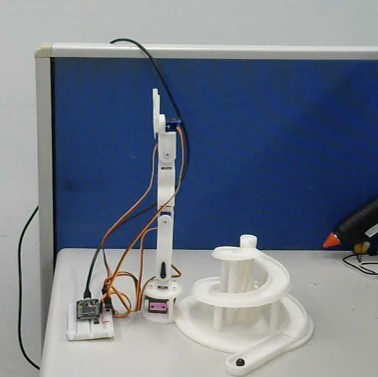
\includegraphics[width=0.4\linewidth]{figures/TB (1).jpg}}
    ~    
    \subcaptionbox
        {移動至黑球位置
        \label{fig:fig-dataset-contrast-after-adjustment}}
        {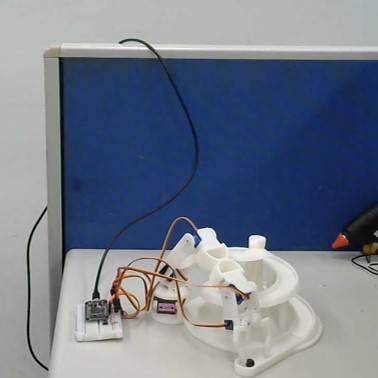
\includegraphics[width=0.4\linewidth]{figures/TB (2).jpg}}
    ~
    \subcaptionbox
        {夾取黑球
        \label{fig:fig-dataset-contrast-after-adjustment}}
        {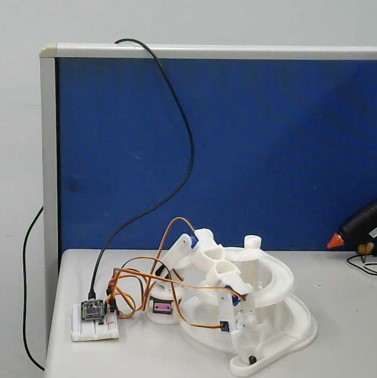
\includegraphics[width=0.4\linewidth]{figures/TB (3).jpg}}
    ~
    \subcaptionbox
        {移動至塔頂位置
        \label{fig:fig-dataset-contrast-after-adjustment}}
        {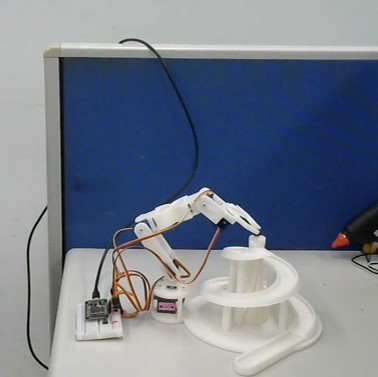
\includegraphics[width=0.4\linewidth]{figures/TB (4).jpg}}
    ~    
    \subcaptionbox
        {放開黑球
        \label{fig:fig-dataset-contrast-after-adjustment}}
        {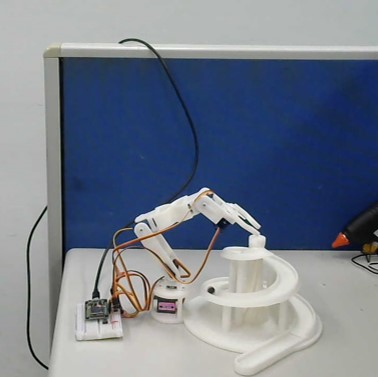
\includegraphics[width=0.4\linewidth]{figures/TB (5).jpg}}
    ~
    \subcaptionbox
        {回到初始位置
        \label{fig:fig-dataset-contrast-after-adjustment}}
        {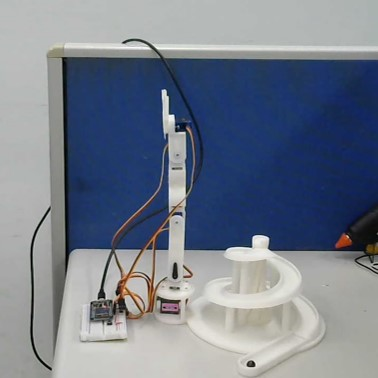
\includegraphics[width=0.4\linewidth]{figures/TB (6).jpg}}   
\caption{實驗一:實驗過程縮圖}
\end{figure}

\section{實驗二:將機械臂用於畫圖}
\subsection{機械結構設計圖}
本實驗的硬體部分使用了3D列印技術,結合小型伺服馬達,
設計了一個畫筆的小型機械臂,以下為此硬體的詳細設計圖紙:
\begin{figure}[htbp]
    \centering
    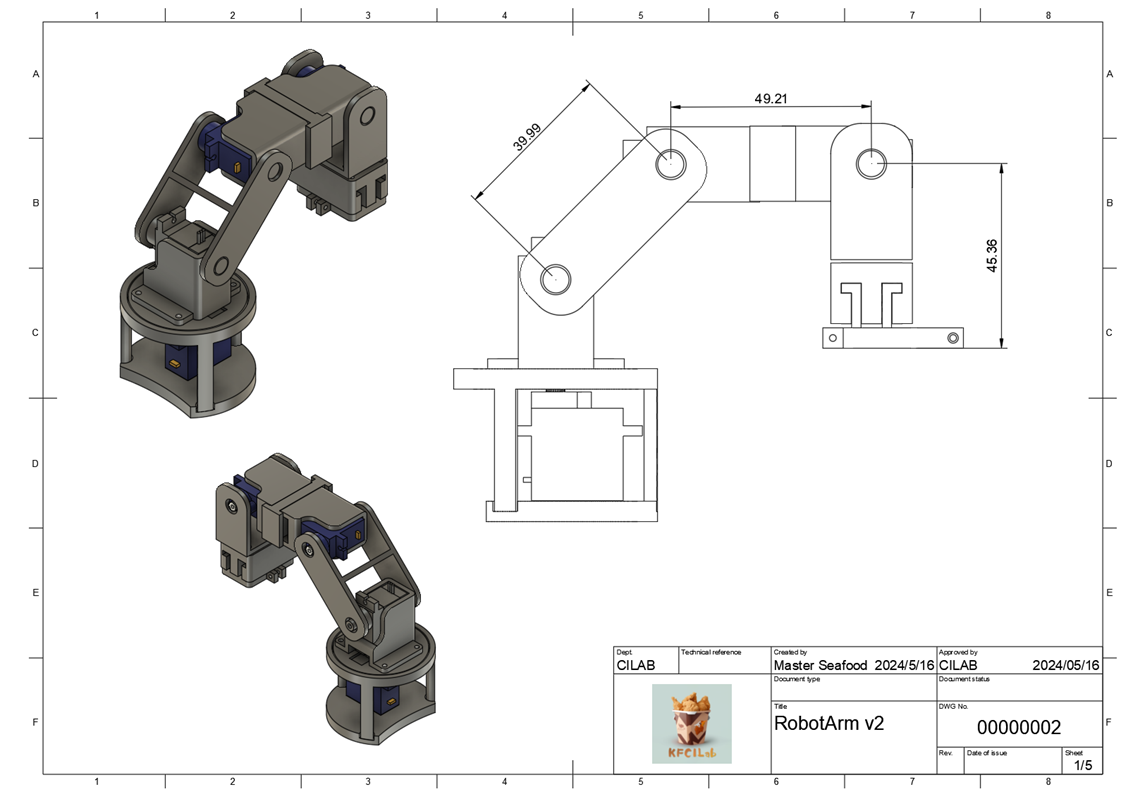
\includegraphics[width=0.9\textwidth]{figures/Armv2 (1).PNG}
    \caption{機械臂版本二設計圖紙 第一頁(單位:mm)}
    %\label{fig:Armv1Drawing_p1}}
\end{figure}

\begin{figure}[htbp]
    \centering
    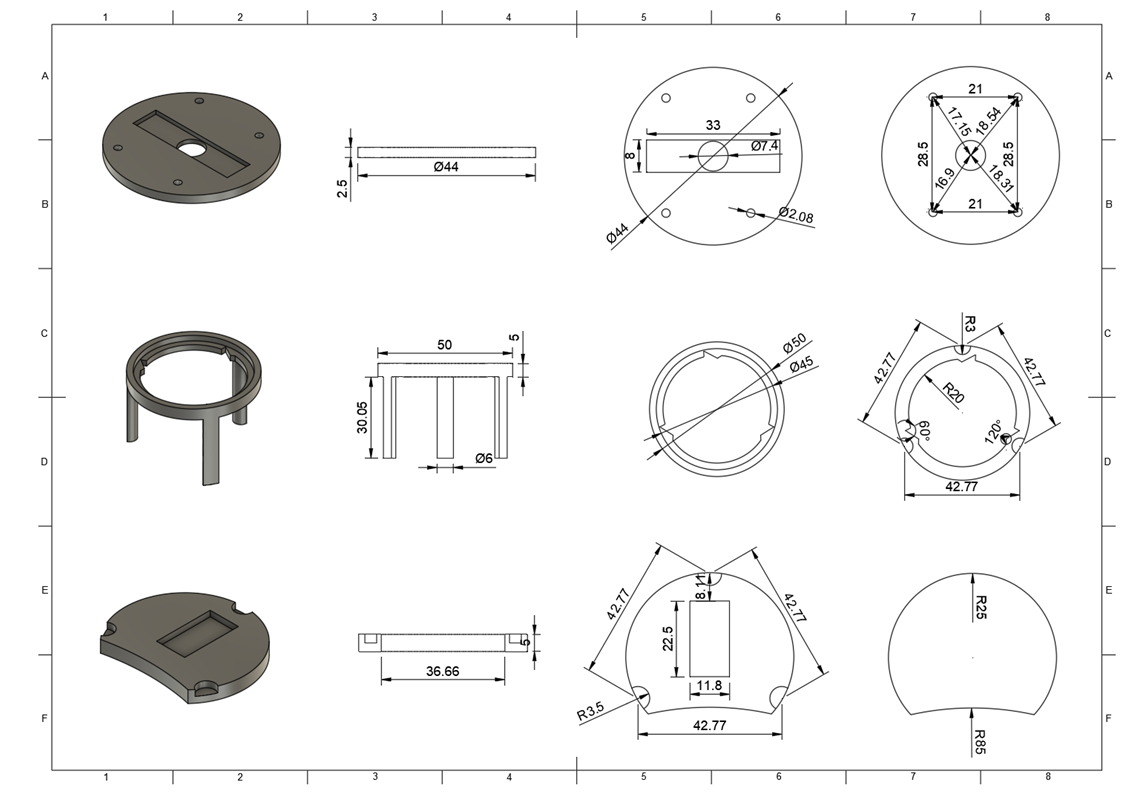
\includegraphics[width=0.9\textwidth]{figures/Armv2 (2).PNG}
    \caption{機械臂版本二設計圖紙 第二頁(單位:mm)}
\end{figure}

\begin{figure}[htbp]
    \centering
    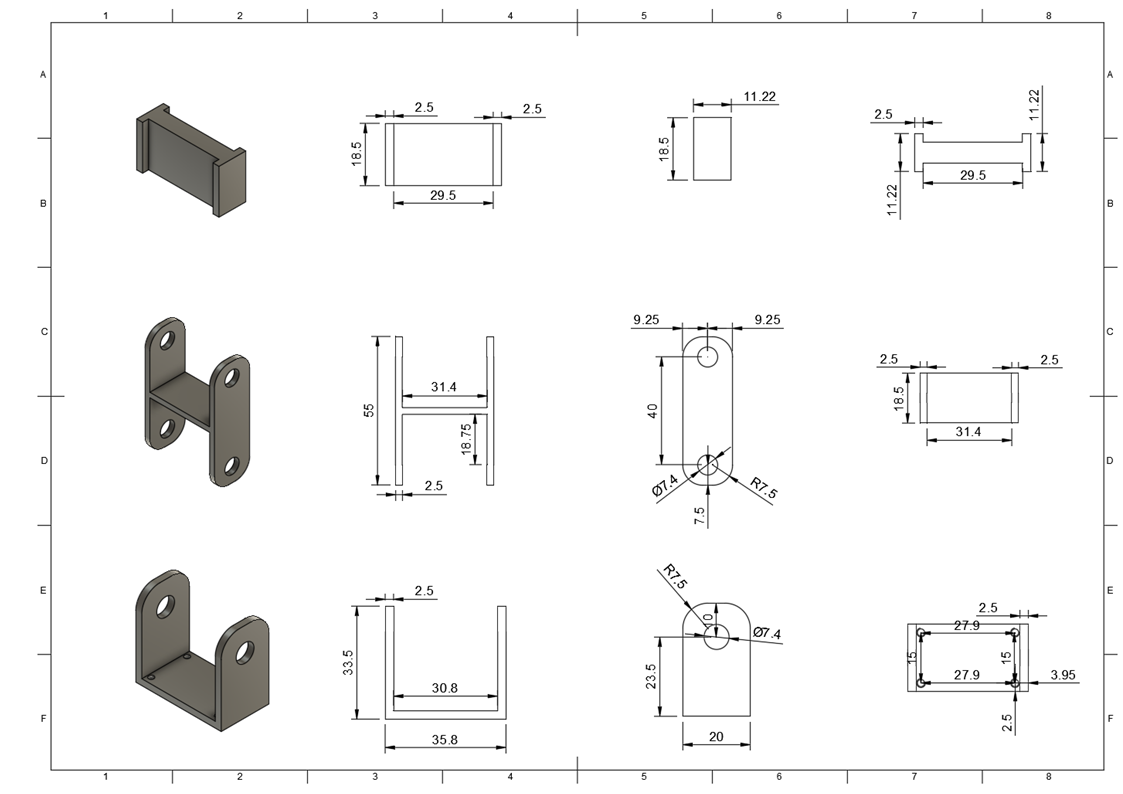
\includegraphics[width=0.9\textwidth]{figures/Armv2 (3).PNG}
    \caption{機械臂版本二設計圖紙 第三頁(單位:mm)}
\end{figure}

\begin{figure}[htbp]
    \centering
    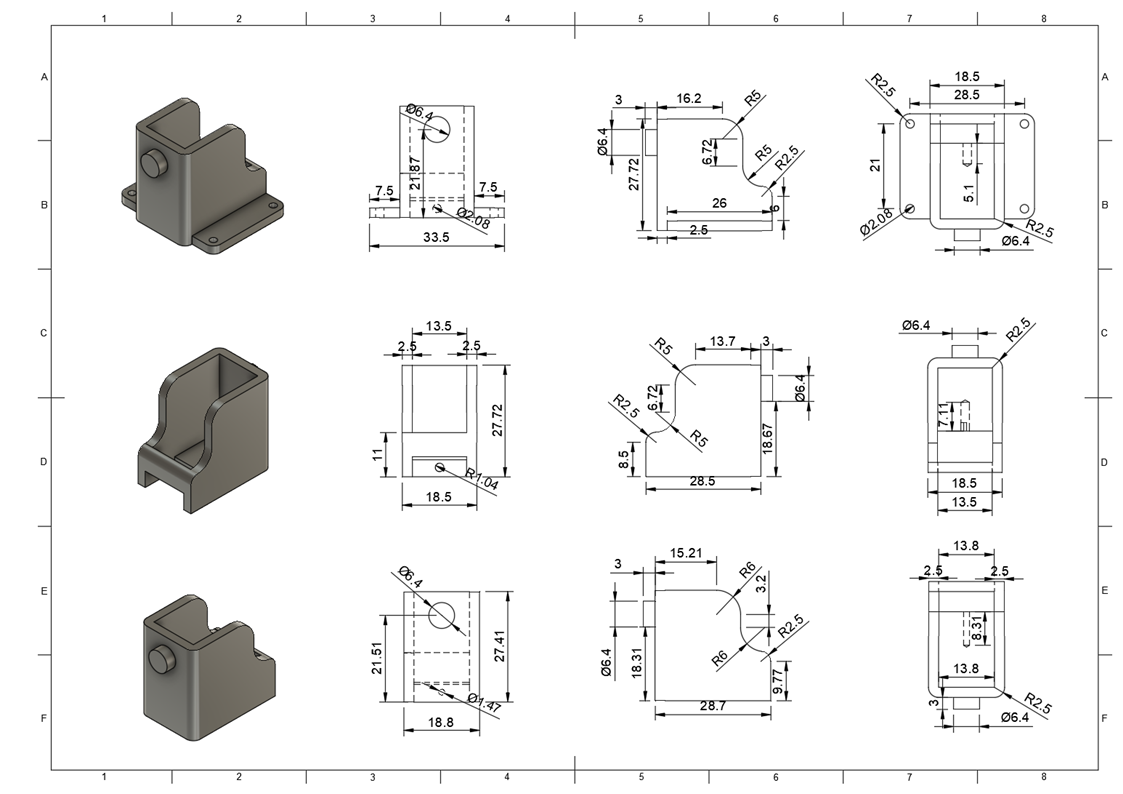
\includegraphics[width=0.9\textwidth]{figures/Armv2 (4).PNG}
    \caption{機械臂版本二設計圖紙 第四頁(單位:mm)}
\end{figure}

\begin{figure}[htbp]
    \centering
    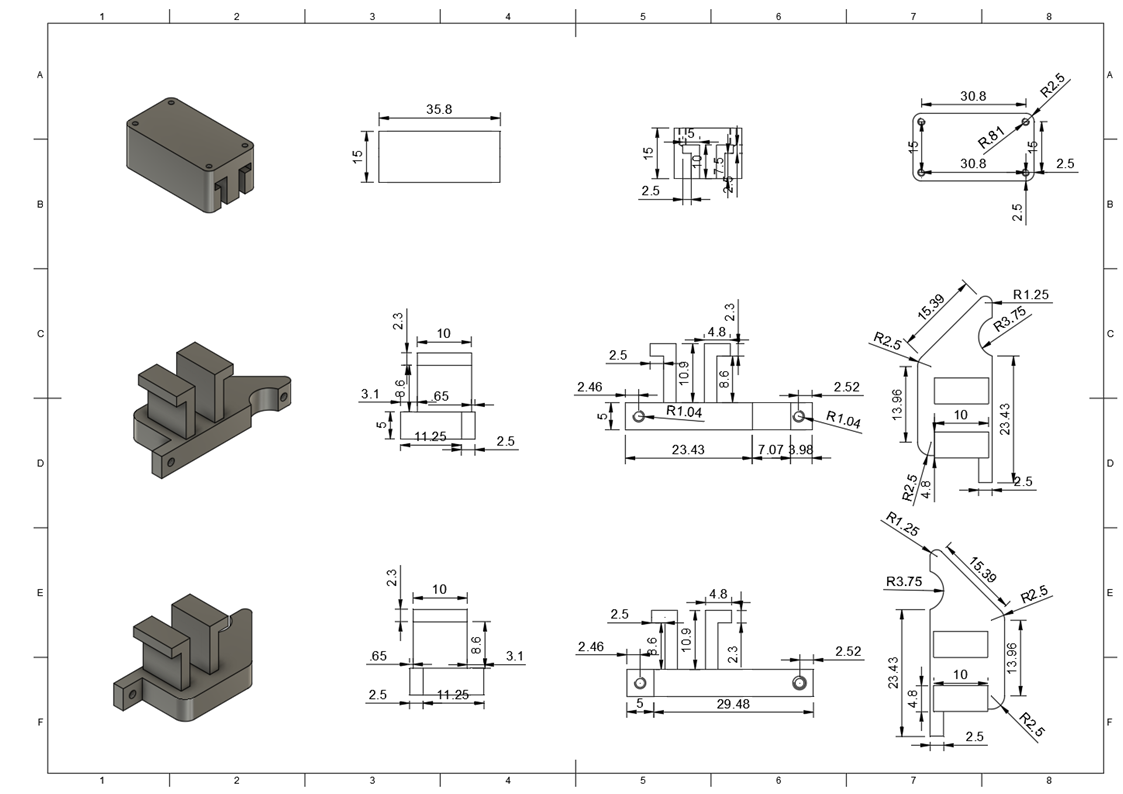
\includegraphics[width=0.9\textwidth]{figures/Armv2 (5).PNG}
    \caption{機械臂版本二設計圖紙 第五頁(單位:mm)}
\end{figure}

\subsection{函數設計}
從實驗一的基礎上,我們改進了機械臂的路徑規劃方法,將其應用於讓機械臂進行畫畫。
此次實驗中,我們簡化了路徑規劃,使大型語言模型在平面座標內進行規劃,
這樣可以降低複雜度,並節省資源。通過這種簡化的路徑規劃方法,
我們能夠更有效地控制機械臂,讓其能夠在紙上或畫布上繪製出預定的圖案。
本實驗將此機器的動作指令簡化為以下函式:

\begin{itemize}
    \item draw(from, to): 由變數from提供的座標,畫至變數to提供的座標。
\end{itemize}
\clearpage
\subsection{下達指令的格式範例}
\begin{listing}[h]
    \begin{minted}[frame=single,
                   framesep=3mm,
                   linenos=true,
                   xleftmargin=21pt,
                   tabsize=4]{js}
    {     
        role: "user",
        content : 
        "The following functions are available:\
        \
        draw(from, to): Let the arm draw a straight line from from to to,\
        such as draw([0, 0], [5, 5]).\
        the limit is[0, 5]\
        \
        Please help me use the above functions to control the robot arm,\
        and do not output other text other than the above functions.\
        (Use "," to separate each step)"
    },
    {
        role: "user", 
        content: "Task: Draw a square."
    }
    \end{minted}
\caption{實驗二:指令格式範例} 
\end{listing}

\begin{listing}[h]
    \begin{minted}[frame=single,
                   framesep=3mm,
                   linenos=true,
                   xleftmargin=21pt,
                   tabsize=4]{js}

    {
        role="assistant",
        content="draw([1, 1], [1, 4]),\
                 draw([1, 4], [4, 4]),\
                 draw([4, 4], [4, 1]),\
                 draw([4, 1], [1, 1])"
    }

    \end{minted}
\caption{實驗二:回傳格式範例} 
\end{listing}

\clearpage
\subsection{實驗結果}

以下為本實驗的實驗過程縮圖與總結:\\

\begin{table}[h]
    \centering
    \caption{實驗結果:Draw a square.}
    \begin{tabular}{ccccc}
    \hline
    大型語言模型 & 總次數 & 成功次數 & 失敗次數 & 成功率 \\
    \hline
    GPT-4o & 10 & 10 & 0 & 1\\
    \hline
    GPT-3.5 Turbo & 10 & 10 & 0 & 1\\
    \hline
    \end{tabular}
\end{table}

\begin{table}[h]
    \centering
    \caption{實驗結果:Draw a triangle.}
    \begin{tabular}{ccccc}
    \hline
    大型語言模型 & 總次數 & 成功次數 & 失敗次數 & 成功率 \\
    \hline
    GPT-4o & 10 & 10 & 0 & 1\\
    \hline
    GPT-3.5 Turbo & 10 & 10 & 0 & 1\\
    \hline
    \end{tabular}
\end{table}

\begin{table}[h]
    \centering
    \caption{實驗結果:Draw a star.}
    \begin{tabular}{ccccc}
    \hline
    大型語言模型 & 總次數 & 成功次數 & 失敗次數 & 成功率 \\
    \hline
    GPT-4o & 10 & 9 & 1 & 0.9\\
    \hline
    GPT-3.5 Turbo & 10 & 5 & 5 & 0.5\\
    \hline
    \end{tabular}
\end{table}

% \begin{table}[h]
%     \centering
%     \caption{實驗結果:Draw a house.}
%     \begin{tabular}{ccccc}
%     \hline
%     大型語言模型 & 總次數 & 成功次數 & 失敗次數 & 成功率 \\
%     \hline
%     GPT-4o & 10 & 7 & 3 & 0.7\\
%     \hline
%     GPT-3.5 Turbo & 10 & 0 & 10 & 0\\
%     \hline
%     \end{tabular}
% \end{table}

在這次實驗中,我們針對上一個實驗中存在的問題進行了改進。首先,我們將複雜的三維空間路徑規劃簡化為平面上的路徑規劃。使的整個控制系統不在需要提供冗長的程式碼與相關條件條件,只需提供特定的圖形,就能驅動機械臂進行繪圖的控制模式,從實驗結果可以看出,這種改進的控制方式不僅大大減少了輸入和回傳的資料量,同時也保持了相當不錯的準確率。這表明此簡化方法在實現高效控制的同時,並未犧牲其性能。因此,我們決定將實驗繼續沿著這個方向進行調整和優化。

\clearpage
\begin{figure}[h]
    \centering
    \subcaptionbox
        {執行畫方形指令
        \label{fig:fig-dataset-contrast-after-adjustment}}
        {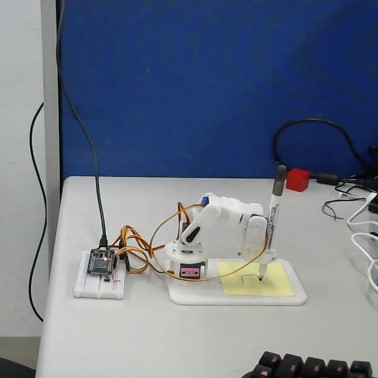
\includegraphics[width=0.4\linewidth]{figures/square_0.jpg}}
    ~    
    \subcaptionbox
        {完成畫方形指令
        \label{fig:fig-dataset-contrast-after-adjustment}}
        {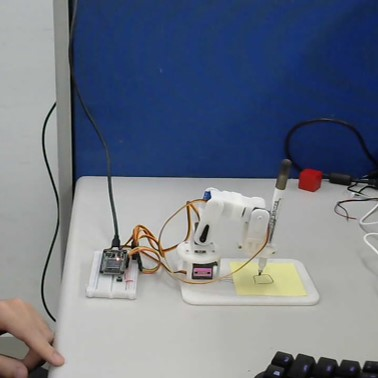
\includegraphics[width=0.4\linewidth]{figures/square_1.jpg}}
    ~
    \subcaptionbox
        {執行畫三角形指令
        \label{fig:fig-dataset-contrast-after-adjustment}}
        {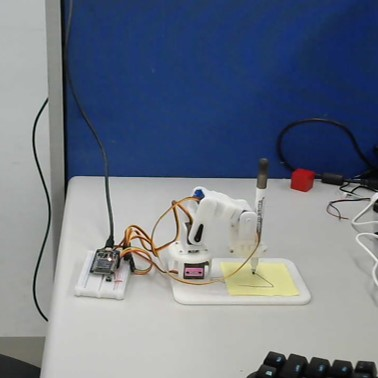
\includegraphics[width=0.4\linewidth]{figures/triangle_0.jpg}}
    ~
    \subcaptionbox
        {完成畫三角形指令
        \label{fig:fig-dataset-contrast-after-adjustment}}
        {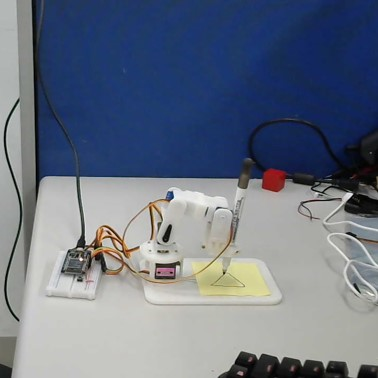
\includegraphics[width=0.4\linewidth]{figures/triangle_1.jpg}}
    ~    
    \subcaptionbox
        {執行畫星形指令
        \label{fig:fig-dataset-contrast-after-adjustment}}
        {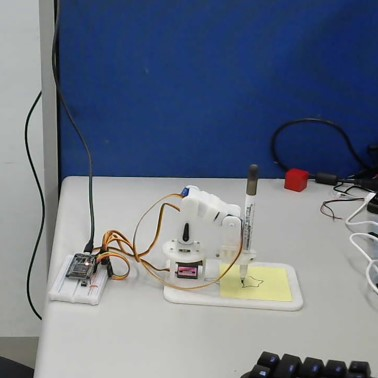
\includegraphics[width=0.4\linewidth]{figures/star_0.jpg}}
    ~
    \subcaptionbox
        {完成畫星形指令
        \label{fig:fig-dataset-contrast-after-adjustment}}
        {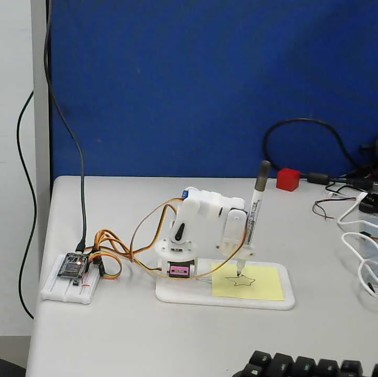
\includegraphics[width=0.4\linewidth]{figures/star_1.jpg}}   
\caption{實驗二:實驗過程縮圖}
\end{figure}

\section{實驗三:機械臂在自動運輸車上的應用}
\subsection{機械結構設計圖}
本實驗將機械臂與自動運輸車、鏡頭等硬體結合,設計了一台裝載機械臂的無人搬運車,以下為此硬體的詳細設計圖紙:
\begin{figure}[htbp]
    \centering
    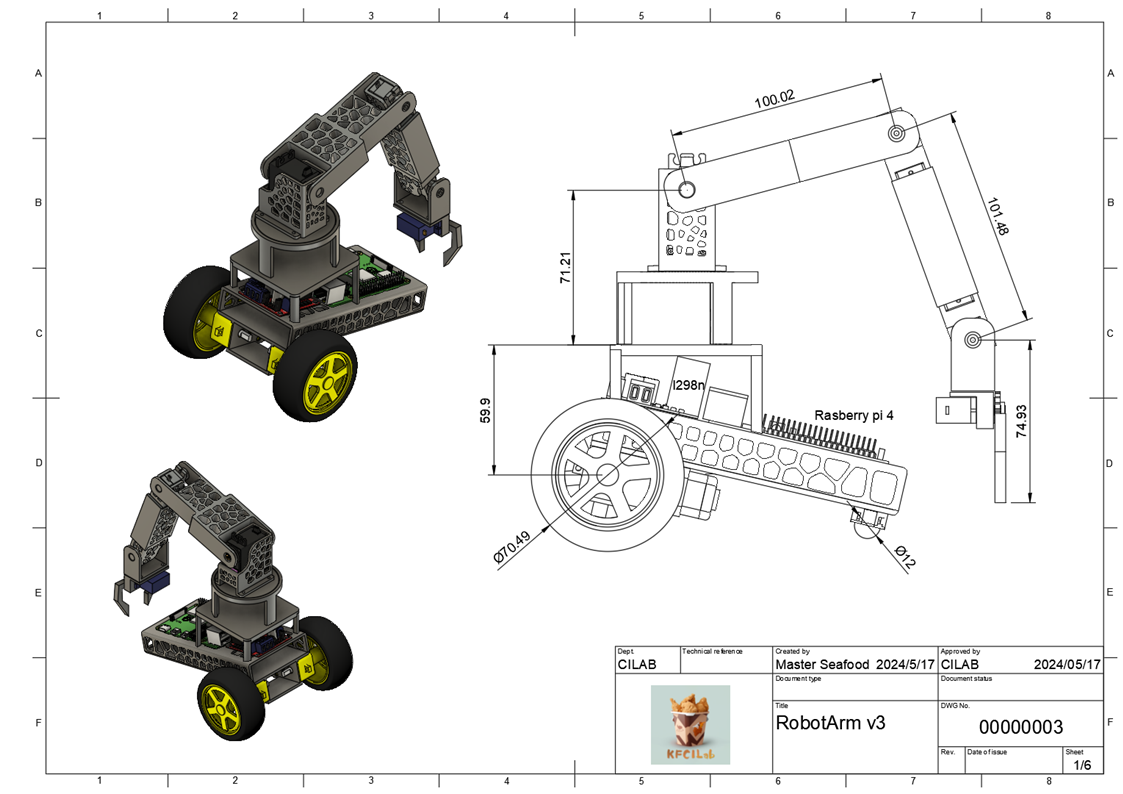
\includegraphics[width=0.9\textwidth]{figures/Armv3 (1).PNG}
    \caption{機械臂版本三設計圖紙 第一頁(單位:mm)}
    %\label{fig:Armv1Drawing_p1}}
\end{figure}

\begin{figure}[htbp]
    \centering
    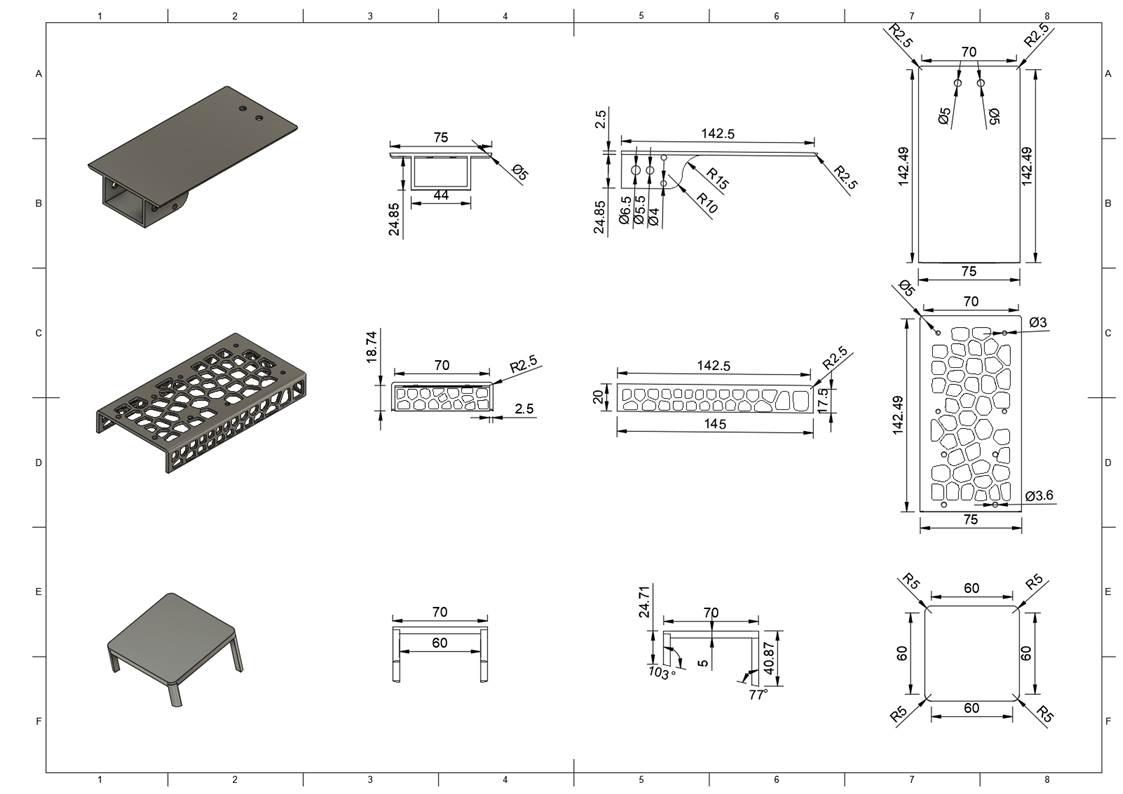
\includegraphics[width=0.9\textwidth]{figures/Armv3 (2).PNG}
    \caption{機械臂版本三設計圖紙 第二頁(單位:mm)}
\end{figure}

\begin{figure}[htbp]
    \centering
    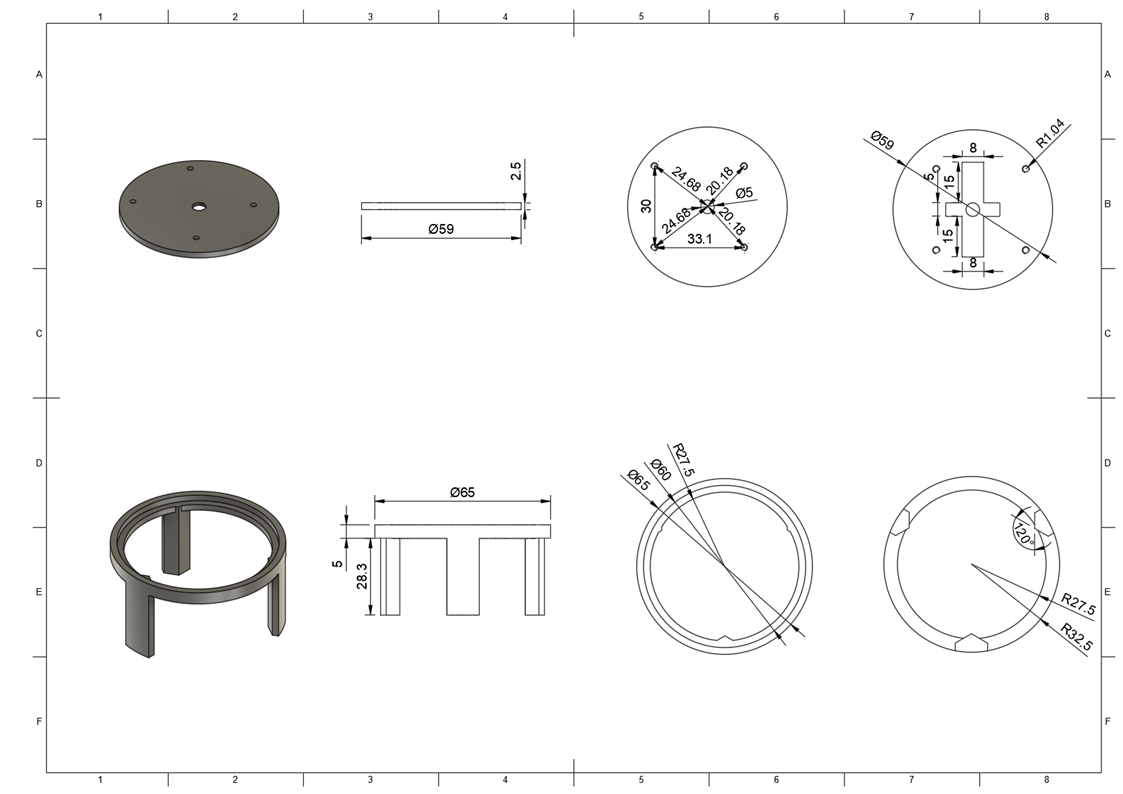
\includegraphics[width=0.9\textwidth]{figures/Armv3 (3).PNG}
    \caption{機械臂版本三設計圖紙 第三頁(單位:mm)}
\end{figure}

\begin{figure}[htbp]
    \centering
    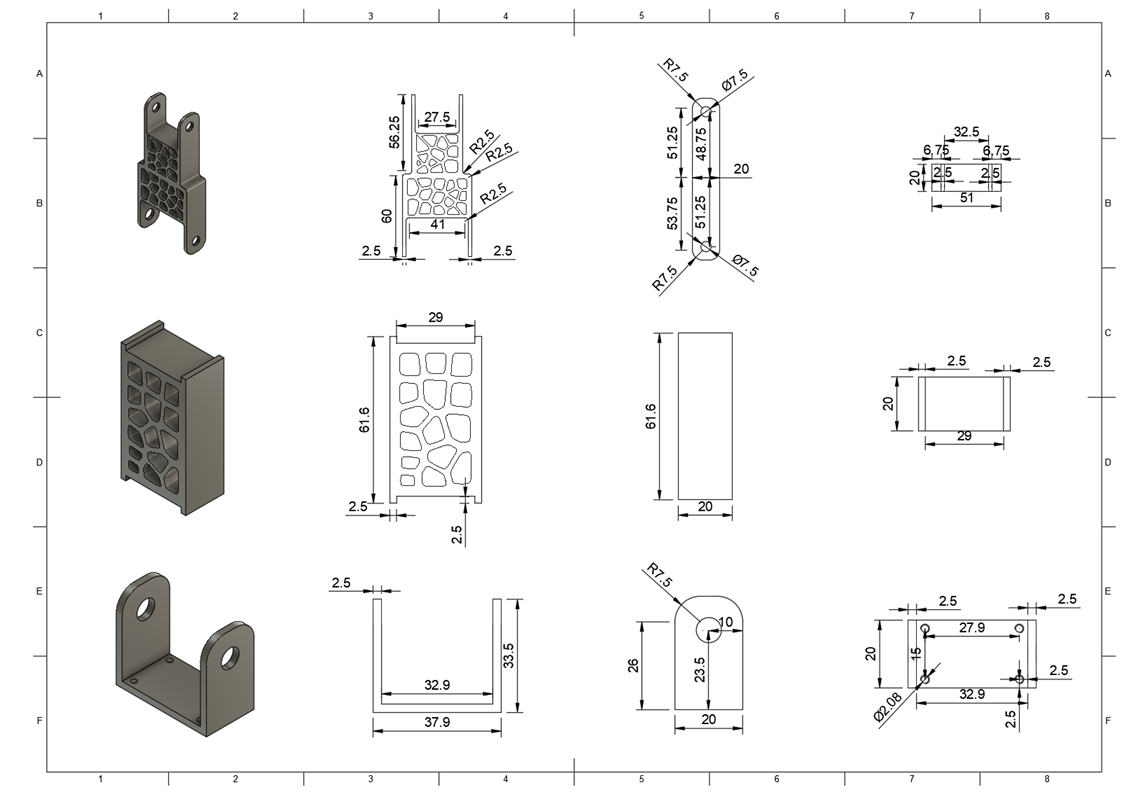
\includegraphics[width=0.9\textwidth]{figures/Armv3 (4).PNG}
    \caption{機械臂版本三設計圖紙 第四頁(單位:mm)}
\end{figure}

\begin{figure}[htbp]
    \centering
    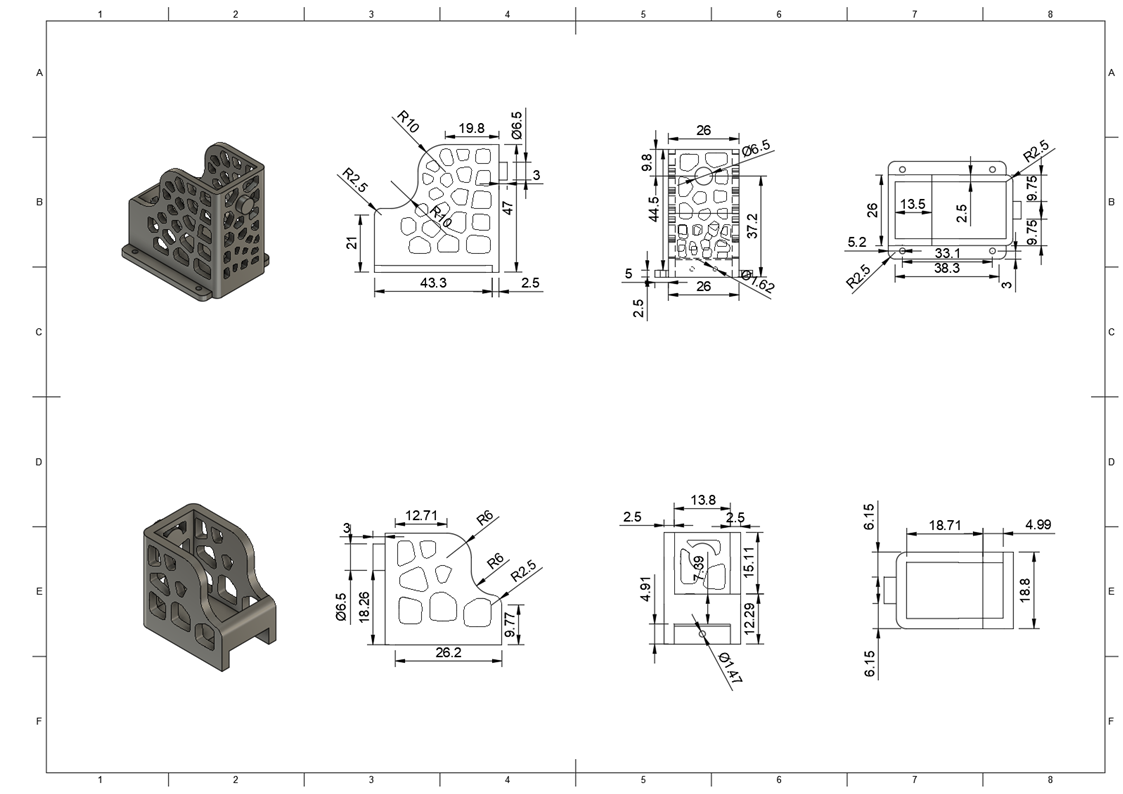
\includegraphics[width=0.9\textwidth]{figures/Armv3 (5).PNG}
    \caption{機械臂版本三設計圖紙 第五頁(單位:mm)}
\end{figure}

\begin{figure}[htbp]
    \centering
    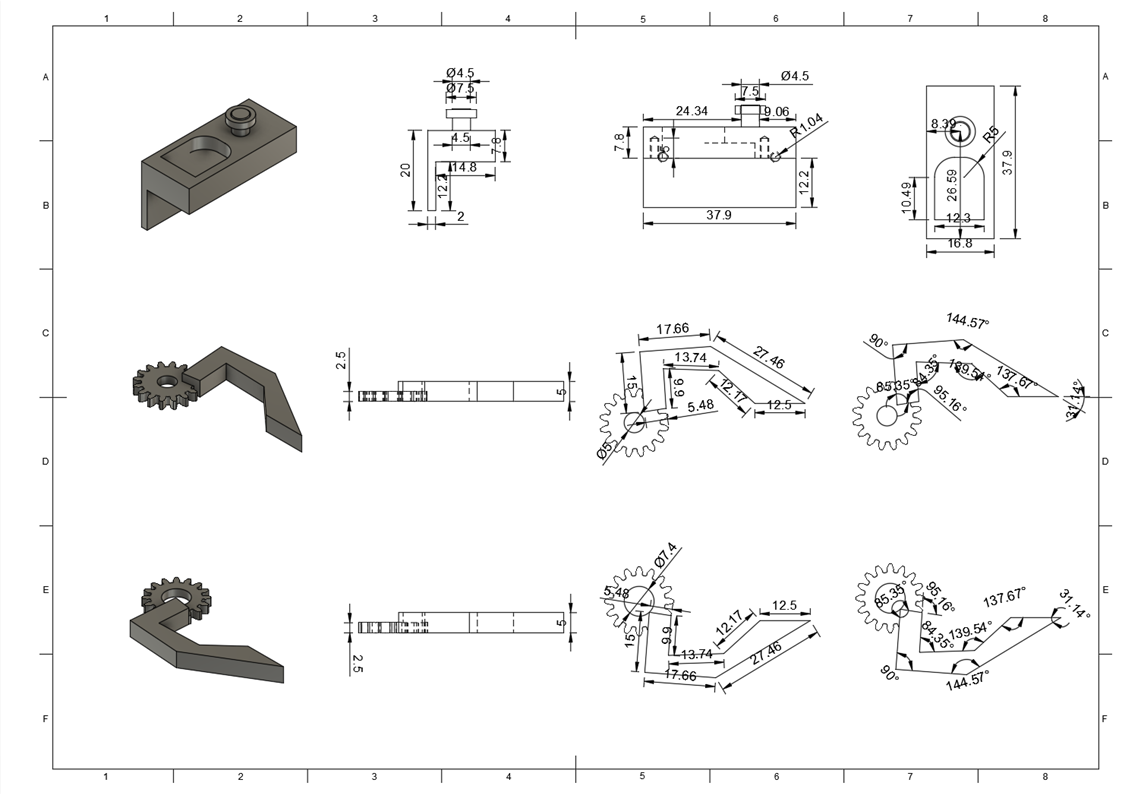
\includegraphics[width=0.9\textwidth]{figures/Armv3 (6).PNG}
    \caption{機械臂版本三設計圖紙 第六頁(單位:mm)}
\end{figure}

\subsection{函數設計}
在前兩個實驗的基礎上,我們進一步改進了控制流程,將機械臂與自動運輸車整合在一起。
這次,我們將控制函式進行細分,並模組化,使得大型語言模型能夠通過簡單的指令來控制機械臂和車輛的行動。
這種模組化的設計不僅降低了指令的複雜度,還減少了資源利用。
最終,我們能夠通過簡單的模組化指令來控制整個系統,
使得機械臂和車輛能夠協同工作,完成更複雜的任務。

\begin{itemize}
    \item find(color): 配合相機定位,驅動輪子尋找動應顏色的方塊。

    \item aim(color): 配合相機定位,驅動機械臂瞄準對應顏色的方塊。

    \item grab(): 驅動機械臂,抓取正下方的物品。

    \item reset(): 驅動機械臂,回到初始位置
\end{itemize}

\newpage
\subsection{下達指令的格式範例}
以下為指令格式:
\begin{listing}[h]
    \begin{minted}[frame=single,
                   framesep=3mm,
                   linenos=true,
                   xleftmargin=21pt,
                   tabsize=4]{js}
    {     
        role: "user",
        content : 
        "The following functions are available:\
        \
        find(color): Let the robot look for a block of a specific color.\
        color option: red, blue.\
        aim(color): Let the robot aim at a block of a specific color.\
        color option: red, blue\
        grab: Make the robot arm grab the block and put it down.\
        reset: Return the robotic arm to its initial position\
        (needs to be executed before each aiming).\
        \
        Please help me use the above functions to control the robot arm,\
        and do not output other text other than the above functions.\
        (Use "," to separate each step)"
    },
    {
        role: "user", 
        content: "Task: Please grab the red block, and then grab the blue block."
    }
    \end{minted}
\caption{實驗三:指令格式範例} 
\end{listing}

\begin{listing}[h]
    \begin{minted}[frame=single,
                   framesep=3mm,
                   linenos=true,
                   xleftmargin=21pt,
                   tabsize=4]{js}

    {
        role="assistant",
        content="find(red), aim(red), grab(), reset(), find(blue), aim(blue), grab()"
    }

    \end{minted}
\caption{實驗三:回傳格式範例} 
\end{listing}

\subsection{實驗結果}
以下為本實驗的實驗過程縮圖與總結:\\


\begin{table}[h]
    \centering
    \caption{實驗結果:Please grab the red block, and then grab the blue block.}
    \begin{tabular}{ccccc}
    \hline
    大型語言模型 & 總次數 & 成功次數 & 失敗次數 & 成功率 \\
    \hline
    GPT-4o & 10 & 9 & 1 & 0.9\\
    \hline
    GPT-3.5 Turbo & 10 & 7 & 3 & 0.7\\
    \hline
    \end{tabular}
\end{table}
在本次實驗中,我們增加了車輪、鏡頭等更多的硬體連動設備。由於每個任務都需要協調各個硬體的運作才能順利完成,我們在撰寫控制程式時,將各個重要指令整理成更加簡化且直觀的獨立函式,這樣可以方便大型語言模型在生成控制指令時直接呼叫這些函式。實驗結果顯示,這種方法取得了非常好的成效,顯著提高了控制指令的生成效率和準確性。然而,由於連動的硬體較多,在呼叫控制函式時難免會發生一些機械性的失誤。例如,鏡頭失真可能導致機械臂瞄準失誤,而車輪的移動則可能導致機械臂在夾取物體時出現掉落的情況。針對這些問題,我們希望在未來進一步優化硬體間的協調機制,以提升系統的穩定性和精確度。

\newpage
\begin{figure}[h]
    \centering
    \subcaptionbox
        {瞄準紅色方塊
        \label{fig:fig-dataset-contrast-after-adjustment}}
        {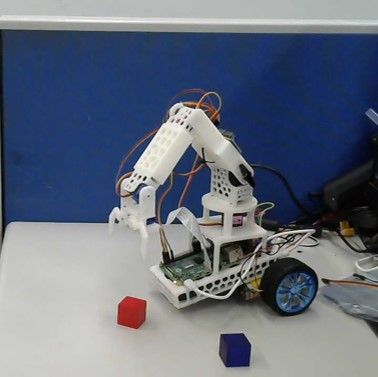
\includegraphics[width=0.4\linewidth]{figures/Exp3 (2)_square.jpg}}
    ~    
    \subcaptionbox
        {夾取紅色方塊
        \label{fig:fig-dataset-contrast-after-adjustment}}
        {\includegraphics[width=0.4\linewidth]{figures/Exp3 (3)_square.jpg}}
    ~
    \subcaptionbox
        {夾取成功
        \label{fig:fig-dataset-contrast-after-adjustment}}
        {\includegraphics[width=0.4\linewidth]{figures/Exp3 (4)_square.jpg}}
    ~
    \subcaptionbox
        {瞄準藍色方塊
        \label{fig:fig-dataset-contrast-after-adjustment}}
        {\includegraphics[width=0.4\linewidth]{figures/Exp3 (5)_square.jpg}}
    ~    
    \subcaptionbox
        {夾取藍色方塊
        \label{fig:fig-dataset-contrast-after-adjustment}}
        {\includegraphics[width=0.4\linewidth]{figures/Exp3 (6)_square.jpg}}
    ~
    \subcaptionbox
        {夾取成功
        \label{fig:fig-dataset-contrast-after-adjustment}}
        {\includegraphics[width=0.4\linewidth]{figures/Exp3 (7)_square.jpg}}   
\caption{實驗三:實驗過程縮圖}
\end{figure}

\end{document}          % 實驗設計與結果
        \documentclass[class=NCU_thesis, crop=false]{standalone}
\begin{document}

\chapter{總結}

\section{結論}

本研究嘗試了機械臂在不同場景中的應用,並分析了其中的控制方法和結果。在實驗中,透過設計機械結構、撰寫控制程式和協調大型語言模型等方式,在進行多次測試後,實驗成功的展示出了機械臂在基本控制、畫圖和自動運輸車上的應用。

在第一個實驗中,我們實現了大型語言模型在機械臂基本控制中的應用,通過給予大型語言模型範例程式,讓其補全其中缺失的路慶規劃部分,
使機械臂能夠精確的完成指定任務。實驗結果顯示,此方法在提高指令生成效率和準確性方面有良好的效果。

第二個實驗中,我們將機械臂用於畫圖,通過簡化指令格式和優化控制函數,成功的實現了簡單圖形的繪製。這展示了此方法在精細操作方面的潛力,並為其在工業設計和藝術創作中的應用提供了可能性。

第三個實驗探討了機械臂在自動運輸車上的應用。實驗結果表明,儘管在硬體連動過程中存在一定的機械性失誤,但通過進一步優化硬體間的協調機制,可以顯著提升系統的穩定性和精確度。

在這些實驗中,我們發現使用大型語言模型進行程式碼生成在控制機器上有很大的潛力。大型語言模型不僅能夠自動生成可執行的控制程式碼,在控制邏輯和處理複雜指令方面也表現出色。
\section{未來展望}

在未來的研究中,我們希望進一步優化機械臂的控制系統,尤其是在硬體協調方面。我們將探索更便利的互動方式,例如通過語音指令直接控制機械臂,使操作更加直觀和方便。讓使用者能夠以自然的語言與機械臂進行溝通和控制,從而大大降低操作的複雜性和學習成本。

此外,我們還計劃利用3D列印技術來製作更多客製化的機械臂及其零部件,並協調整合更多的硬體設備。使我們能夠快速設計和生產符合特定應用需求的機械臂,從而滿足不同行業和應用場景的需求。

另外,我們將研究和開發更多模組化的機械臂控制函式庫,以便大型語言模型能夠直接使用這些函式庫進行機械臂的控制。這些模組化函式庫將包含多種預先定義的操作和功能,使得開發者可以輕鬆地構建和定制機械臂的操作流程,進一步提升開發效率和彈性。

總之,本研究展示了智慧機器與大型語言模型在多種應用場景中的廣闊前景。我們期待未來能夠通過技術創新和多設備整合,進一步擴展大型語言模型在機器控制上的應用範圍,推動機械臂技術向更加智能化、人性化和客製化的方向發展。
\end{document}      % 結論
    %     \documentclass[class=NCU_thesis, crop=false]{standalone}
\usepackage{showexpl}

\begin{document}

\chapter{章名(章節示例)}
章內容內容內容內容內容 \\
內容內容內容

\section{節名}
節內容內容內容內容內容 \\
內容內容內容

\subsection{小節名}
內容內容內容 \\
內容內容內容

\subsubsection{小小節}
內容內容內容 \\
內容內容內容

\paragraph{段}
內容內容內容 \\
內容內容內容

\subparagraph{小段}
內容內容內容 \\
內容內容內容


\chapter{文字}
第一行。
仍是第一行。 \\
第二行。


\chapter{圖片}
\section{插入單一圖片}
\fig[0.15][fig:label_test][!hbt]{logo-Linux.png}[caption][short caption]

\section{插入多張圖片}
\begin{figure}[!hbt]
    %\captionsetup[subfigure]{labelformat=empty} % 完全隱藏圖號
    \centering
    \subcaptionbox
        {caption\_1
        \label{fig:subfig_fig1}}
        {\includegraphics[width=0.3\linewidth]{fig1.png}}
    ~
    \subcaptionbox
        {caption\_2
        \label{fig:subfig_fig2}}
        {\includegraphics[width=0.3\linewidth]{fig2.eps}}
    \vspace{\baselineskip} % 分隔上下列
    \subcaptionbox
        {caption\_3
        \label{fig:subfig_fig3}}
        {\includegraphics[width=0.6\linewidth]{fig3.png}}
    \caption{caption, 使用 \subref{fig:subfig_fig2}取得子圖(Debian)編號 }
    \label{fig:label}
\end{figure}


\chapter{表格}
\section{一般表格}
\begin{table}[h]
    \centering
    \caption{Solution}
    \begin{tabular}{| l | l |}
        \hline
        Component & Concentration(mM) \\ \hline
        \ce{NaCl} & 118.0 \\ \hline
    \end{tabular}
\end{table}

\section{自動折行表格}
\begin{table}[h]
    \centering
    \begin{tabularx}{\textwidth}{| l | X |}
        \hline
        short & short short \\ \hline
        long & long long long long long long long long long long  long long long long long long long long long long\\ \hline
    \end{tabularx}
\end{table}

\end{document}
    \backmatter          % book class 預設\backmatter 在\appendix 後面。因此.cls修改過\appendix 定義
        % This file has 3 types bibliography management, 
% \bibManType in config.tex choose it.
% 0. Embedded: write \bibitem in {thebibliography} environment.
% 1. BibTeX: Change bib files in \bibliography{}
% 2. biber / BibLaTeX: Add bibliography by \addbibresource{bibfile.bib} in macros_preamble.tex

\documentclass[class=NCU_thesis, crop=false]{standalone}

\begin{document}

\ifcase \bibManType 
    % 0 == Embedded %%%%%%%%%%%%%%%%%%%%%%%%%%%%%%%%%%%%%%%
    {\bibFontStyle\setstretch{\bibLineStretch}
    \begin{thebibliography}{99}

    \bibitem{cite_key_1}
        bibliography item detail.

    \bibitem{_sppmg/tw_thesis_template_????}
        TW\_Thesis\_Template,
        sppmg,
        \url{https://github.com/sppmg/TW_Thesis_Template},
        Embedded bibliography demo.

    \end{thebibliography}
    }
    
\or
    % 1 == BibTeX %%%%%%%%%%%%%%%%%%%%%%%%%%%%%%%%%%%%%%%%%
    \bibliographystyle{\bibStyle}
    {\bibFontStyle\setstretch{\bibLineStretch}
        \bibliography{demo} % {sample_1,sample_2,...,sample_n}
        % Note the lack of whitespace between the commas and the next bib file.
    }
\or

    % 2 == biber / BibLaTeX %%%%%%%%%%%%%%%%%%%%%%%%%%%%%%%
    \printbibliography[title = {參考文獻}, heading = bibnumbered]
\fi



\end{document}
    % \appendix
    %     \documentclass[class=NCU_thesis, crop=false]{standalone}
\begin{document}

\chapter{裝置列表}

\begin{table}[!h]
    \centering
    \begin{tabularx}{\textwidth}{|l|l|X|}
        \hline
        裝置	     & 型號      & 說明 \\ \hline
        Linux    & Debian 9 & 世界好用的作業系統 \\ \hline
        Windows  & 10       & 防止人腦老化的工具 \\ \hline
    \end{tabularx}
    \caption{裝置列表}
    \label{table:list_device}
\end{table}

\end{document}
    %     \documentclass[class=NCU_thesis, crop=false]{standalone}
\begin{document}

\definecolor{Gray3}{gray}{0.8}

\chapter{Solutions}

\section{The solution}
\begin{table}[!h]
    \centering
    \begin{tabular}{| l | l |}
        \hline
        Component & Concentration(mM) \\ \hline
        \rowcolor{Gray3}
        \ce{NaCl} & 1.0 \\ \hline
        \ce{CaCl_2} & 2.0 \\ \hline
        \rowcolor{Gray3}
        \ce{NaCl} & 1.0 \\ \hline
        \ce{CaCl_2} & 2.0 \\ \hline
    \end{tabular}
    \caption{The solution}
\end{table}
\end{document}
    %     \documentclass[class=NCU_thesis, crop=false]{standalone}
\begin{document}
% Here demo instert whole code file. You can only insert code directly, 
% please read my tutorial or document of listings package.
% code style set in macros_preamble already.
% Supported language please read document of listings package or
% https://www.sharelatex.com/learn/Code_listing#!#Supported_languages

\chapter{程式碼}
\section{C}
\lstinputlisting[language=C]{hello_world_c.c}

\section{Matlab}
\lstinputlisting[language=matlab]{hello_world_matlab.m}

\section{IDL}
\lstinputlisting[language=IDL]{hello_world_idl.pro}
\end{document}

    %     \documentclass[class=NCU_thesis, crop=false]{standalone}

\begin{document}
\chapter{自動填單}
這裡試著幫各位自動填入部份資訊,其餘打勾、日期請手寫。有字體大小不符、位置歪掉等問題的話,請修改 appendix\_letter\_NCU.tex後直接編譯生成文件。

appendix\_letter\_NCU.tex中,每個句子(文字項目)都是獨立的大小與位置。 大小可由\textbackslash{}fs,調整。
\footnote{\textbackslash{}fs 使用 \textbackslash{}fontsize 做無級調整,並固定單行高度。 }
位置可由\textbackslash{}placetextbox 調整。語法如下:
\begin{lstlisting}[style=LatexStyle,caption={}]
\placetextbox{x(mm)}{y(mm)}
\end{lstlisting}
單位使用mm ,(0,0)位於左下角。建議調整時將``colorgrid''加入documentclass選項。(加入子檔的即可)
\begin{lstlisting}[style=LatexStyle,caption={}]
\documentclass[class=NCU_thesis, crop=false, colorgrid]{standalone}
\end{lstlisting}
colorgrid 將顯示格線(一小格是\SI{5}{\milli\metre})。

\begin{center}
{ \noindent\color{red}\bfseries\Large NCU English letters in the NCU\_en}
\end{center}

%%%%%%%%%%%%%%%%%%%%%%%%%%%%%%%%

% define \mprof 
\ExplSyntaxOn
    % Copy prof. list from config.tex
    \clist_gclear_new:N \g_sppmg_profs_cl
    \clist_gset:NV \g_sppmg_profs_cl \profs
    \clist_gpop:NNTF \g_sppmg_profs_cl \l_tmpa_tl {}{ \tl_clear:N \l_tmpa_tl}
    \cs_gset_eq:NN \mprof \l_tmpa_tl
\ExplSyntaxOff

\cleardoublepage
\pagestyle{empty}
\sffamily
% ------------------------------

% % 碩博士論文電子檔授權書
\IfFileExists{\letterAuthEl}{
\cleardoublepage\thispagestyle{empty}
\includepdf[pagecommand={   \placetextbox{100}{120}{\fs{17}\title}%
                            \placetextbox{95}{109}{\fs{17}\mprof}%
                            \placetextbox{69}{98}{\fs{17}\deptshort} }]%
{\letterAuthEl}}{}

% 碩博士紙本論文延後公開/下架申請書。(如需延後公開者,才需要裝訂於論文內頁)
\IfFileExists{\letterPubReq}{
\cleardoublepage\thispagestyle{empty}
\includepdf[pagecommand={   \placetextbox{128}{270}{\fs{17}\author}%
                            \placetextbox{70}{258}{\fs{17}\deptshort}%
                            \placetextbox{100}{233}{\fs{17}\title}%
                            \placetextbox{90}{219.3}{\fs{17}\mprof} }]%
{\letterPubReq}}{}

% 指導教授推薦書
\IfFileExists{\letterRecom}{
\cleardoublepage\thispagestyle{empty}
\includepdf[pagecommand={   \placetextbox{50}{159}{\fs{22}\deptshort}%
                            \placetextbox{118}{159}{\fs{22}\author}%
                            \placetextbox{105}{144}{\fs{22}\title}}%
]{\letterRecom}}{}

% 口試委員審定書
\IfFileExists{\letterVerif}{
\cleardoublepage\thispagestyle{empty}
\includepdf[pagecommand={   \placetextbox{63}{200.5}{\fs{22}\deptshort}%
                            \placetextbox{145}{200.5}{\fs{22}\author}%
                            \placetextbox{100}{170}{\fs{22}\title}}%
]{\letterVerif}}{}

% ------------------------------
\pagestyle{fancy}
\end{document}
\end{document}